\documentclass{scrartcl}  
% Include all project wide packages here.
\usepackage{fullpage}
\usepackage{polyglossia}
\setmainlanguage{dutch}
\usepackage{csquotes}
\usepackage{graphicx}
\usepackage{epstopdf}
\usepackage{pdfpages}
\usepackage{caption}
\usepackage[list=true]{subcaption}
\usepackage{float}
%\usepackage{mathtools}
\usepackage{standalone}
\usepackage{import}
\usepackage{tocloft}
\usepackage{wrapfig}
\usepackage{authblk}
\usepackage{array}
\usepackage{booktabs}
\usepackage[toc,page,title,titletoc]{appendix}
\usepackage{xunicode}
\usepackage{amsmath}
\usepackage{fontspec}
\usepackage{unicode-math}
\usepackage[
    backend=bibtexu,
	texencoding=utf8,
bibencoding=utf8,
    style=ieee,
    sortlocale=nl_NL,
    language=auto
]{biblatex}
\usepackage{listings}
\newcommand{\includecode}[3][c]{\lstinputlisting[caption=#2, escapechar=, style=#1]{#3}}
\newcommand{\superscript}[1]{\ensuremath{^{\textrm{#1}}}}
\newcommand{\subscript}[1]{\ensuremath{_{\textrm{#1}}}}


\newcommand{\chapternumber}{\thechapter}
\renewcommand{\appendixname}{Bijlage}
\renewcommand{\appendixtocname}{Bijlagen}
\renewcommand{\appendixpagename}{Bijlagen}

\usepackage[hidelinks]{hyperref} %<--------ALTIJD ALS LAATSTE
  
\renewcommand{\familydefault}{\sfdefault}

\setmainfont[Ligatures=TeX]{Myriad Pro}
\setmathfont{Asana Math}
\setmonofont{Lucida Console}

\usepackage{titlesec, blindtext, color}
\definecolor{gray75}{gray}{0.75}
\newcommand{\hsp}{\hspace{20pt}}
\titleformat{\chapter}[hang]{\Huge\bfseries}{\chapternumber\hsp\textcolor{gray75}{|}\hsp}{0pt}{\Huge\bfseries}
\renewcommand{\familydefault}{\sfdefault}
\renewcommand{\arraystretch}{1.2}
\setlength\parindent{0pt}

%For code listings
\definecolor{black}{rgb}{0,0,0}
\definecolor{browntags}{rgb}{0.65,0.1,0.1}
\definecolor{bluestrings}{rgb}{0,0,1}
\definecolor{graycomments}{rgb}{0.4,0.4,0.4}
\definecolor{redkeywords}{rgb}{1,0,0}
\definecolor{bluekeywords}{rgb}{0.13,0.13,0.8}
\definecolor{greencomments}{rgb}{0,0.5,0}
\definecolor{redstrings}{rgb}{0.9,0,0}
\definecolor{purpleidentifiers}{rgb}{0.01,0,0.01}


\lstdefinestyle{csharp}{
language=[Sharp]C,
showspaces=false,
showtabs=false,
breaklines=true,
showstringspaces=false,
breakatwhitespace=true,
escapeinside={(*@}{@*)},
columns=fullflexible,
commentstyle=\color{greencomments},
keywordstyle=\color{bluekeywords}\bfseries,
stringstyle=\color{redstrings},
identifierstyle=\color{purpleidentifiers},
basicstyle=\ttfamily\small}

\lstdefinestyle{c}{
language=C,
showspaces=false,
showtabs=false,
breaklines=true,
showstringspaces=false,
breakatwhitespace=true,
escapeinside={(*@}{@*)},
columns=fullflexible,
commentstyle=\color{greencomments},
keywordstyle=\color{bluekeywords}\bfseries,
stringstyle=\color{bluestrings},
identifierstyle=\color{purpleidentifiers}
}

\lstdefinestyle{vhdl}{
language=VHDL,
showspaces=false,
showtabs=false,
breaklines=true,
showstringspaces=false,
breakatwhitespace=true,
escapeinside={(*@}{@*)},
columns=fullflexible,
commentstyle=\color{greencomments},
keywordstyle=\color{bluekeywords}\bfseries,
stringstyle=\color{redstrings},
identifierstyle=\color{purpleidentifiers}
}

\lstdefinestyle{xaml}{
language=XML,
showspaces=false,
showtabs=false,
breaklines=true,
showstringspaces=false,
breakatwhitespace=true,
escapeinside={(*@}{@*)},
columns=fullflexible,
commentstyle=\color{greencomments},
keywordstyle=\color{redkeywords},
stringstyle=\color{bluestrings},
tagstyle=\color{browntags},
morestring=[b]",
  morecomment=[s]{<?}{?>},
  morekeywords={xmlns,version,typex:AsyncRecords,x:Arguments,x:Boolean,x:Byte,x:Char,x:Class,x:ClassAttributes,x:ClassModifier,x:Code,x:ConnectionId,x:Decimal,x:Double,x:FactoryMethod,x:FieldModifier,x:Int16,x:Int32,x:Int64,x:Key,x:Members,x:Name,x:Object,x:Property,x:Shared,x:Single,x:String,x:Subclass,x:SynchronousMode,x:TimeSpan,x:TypeArguments,x:Uid,x:Uri,x:XData,Grid.Column,Grid.ColumnSpan,Click,ClipToBounds,Content,DropDownOpened,FontSize,Foreground,Header,Height,HorizontalAlignment,HorizontalContentAlignment,IsCancel,IsDefault,IsEnabled,IsSelected,Margin,MinHeight,MinWidth,Padding,SnapsToDevicePixels,Target,TextWrapping,Title,VerticalAlignment,VerticalContentAlignment,Width,WindowStartupLocation,Binding,Mode,OneWay,xmlns:x}
}

%defaults
\lstset{
basicstyle=\ttfamily\small,
extendedchars=false,
numbers=left,
numberstyle=\ttfamily\tiny,
stepnumber=1,
tabsize=4,
numbersep=5pt
} 
\addbibresource{../../library/bibliography.bib}

\author{Robin Hes (4236815) \and Jorden Kerkhof (4232461)}

\title{EPO3-1 - Opdracht 4: Unified Model Parameters}
\subtitle{EE2821 - TU Delft}
\date{3 oktober 2013}

\begin{document}
\maketitle

\section*{Abstract}
In dit verslag zal blijken dat het mogelijk is, om met een set berekende parameters voor een CMOS-transistor die allen meer dan 60\% afwijken van een set gegeven parameters, toch een simulatie met een gemiddelde afwijking van minder dan 5\%, tegenover een SPICE-model, uit te voeren. Daarmee blijkt het unified transistor model van Rabaey een goede representatie die in een aantal gevallen bruikbaar is voor handmatige analyse.

\newpage
\label{sec:ump-abstr}

\tableofcontents

\section{Inleiding}
\label{sec:ump-inl}
Voor deze opdracht was het de bedoeling om meer inzicht te krijgen in het gedrag en de werking van MOS transistoren. Er moet een model van de transistoren worden gesimuleerd in PSPICE. Vervolgens moesten de resultaten hiervan worden geanalyseerd en juist worden geinterpreteerd. Iedereen kreeg een eigen opdracht met wat er onderzocht moest worden aan de transistor. Wij hadden de opdracht Unified Model Parameters.

\newpage
\section{Probleemstelling}
\label{sec:ump-prob}
De probleemstelling is zoals gegeven in opdracht 4: \\
\textit{
``Bepaal voor een NMOS transistor de volgende parameters uit het unified transistor model van Rabaey:
$V_{T0}$ \quad $V_{DSAT}$ \quad $k'$ \quad $\lambda$ \\
Vergelijk vervolgens de uitkomsten van het Unified Model met de SPICE simulaties zoals bijvoorbeeld
gedaan is in figuur 3.25. Vergelijk ook de gevonden waarde met waarden van de technologie uit het Rabaey
boek en bediscussieer het verschil in het licht van de discussie over schaling in sectie 3.5 van het Rabaey
boek. Vergelijk ook met de parameters van de gegeven SPICE modellen van de SoG technologie en bediscussieer
eventuele verschillen.''
}
\cite[4]{epo3-opdracht-4}


\section{Theorie}
\label{sec:ump-theorie}
In SPICE-simulaties wordt uiteraard een model gebruikt, dat een werkelijke transistor zo goed mogelijk nabootst. Een computer rekent immers veel sneller dan een mens en dus is de complexiteit van het model een minder groot probleem. Voor handmatige analyse van een CMOS-transistor is het echter wenselijk om een model te hebben dat ook voor de mens te gebruiken is.
Het unified transistormodel van Rabaey biedt hier een uitkomst. Het model beschrijft, met slechts een enkele vergelijking, de drainstroom $I_{D}$ door de transistor, aan de hand van een vrij beperkt aantal parameters. De drainstroom wordt gemodelleerd in de drie verschillende werkgebieden waarin de transistor zich kan bevinden, wanneer deze in geleiding is, afhankelijk van de spanning over drain en source ($V_{DS}$). Daarnaast beschrijft het model de effecten van velocity saturation.
De vergelijking voor $I_{D}$, zoals gegeven door Rabaey, is als volgt:

\begin{equation} \label{eq:ump-cmos-model-rab}
	I_{D} = k' \frac{W}{L} (V_{GT}V_{min} - \frac{V_{min}^2}{2})(1 + \lambda V_{DS})	
\end{equation}

Waarbij geldt dat: \\
$$V_{min} = min(V_{GT}, V_{DS}, V_{DSAT})$$
$$V_{GT} = V_{GS} - V_{T}$$
$$V_{T} = V_{T0} + \gamma ( \sqrt{|-2\phi_{F} + V_{SB}|} - \sqrt{|-2\phi_{F}|} )$$
\cite[101]{rabaey-integrated-circuits}\\

Hierin hangen $V_{GS}$, $V_{DS}$ en $V_{SB}$ af van de situatie en zijn $W$, $L$, $k'$, $V_{T0}$, $V_{DSAT}$, $\gamma$, $\lambda$ en $\phi_{F}$ eigenschappen van de transistor. Tevens kan de term $k' \frac{W}{L}$ genoteerd worden als $k$, deze notatie wordt in dit verslag waar dat mogelijk is gebruikt.
\\

In sectie~\ref{sec:ump-methode} zal de gebruikte methode uiteen gezet worden, om relevante parameters ($k'$, $V_{T0}$, $V_{DSAT}$ en $\lambda$) uit het gegeven model te bepalen, aan de hand van een SPICE-simulatie. Met deze parameters kan vervolgens gerekend worden aan de MOS-transistors uit de bij EPO-3 gebruikte Sea-of-Gates-chip.

\section{Methode}
\label{sec:ump-methode}
\subsection{Simulatie}
\label{subsec:ump-methode-sim}

Om de voor deze opdracht vereiste parameters te bepalen is er als eerste data nodig om deze uit te bepalen. Dit kunnen metingen aan een daadwerkelijke transistor zijn, maar voor het doel van deze opdracht volstaat het om gegevens uit een SPICE-simulatie te gebruiken. Daarom simuleren we het onderstaande circuit (figuur~\ref{fig:ump-sim-circuit}).

\begin{figure}[H]
	\centering
	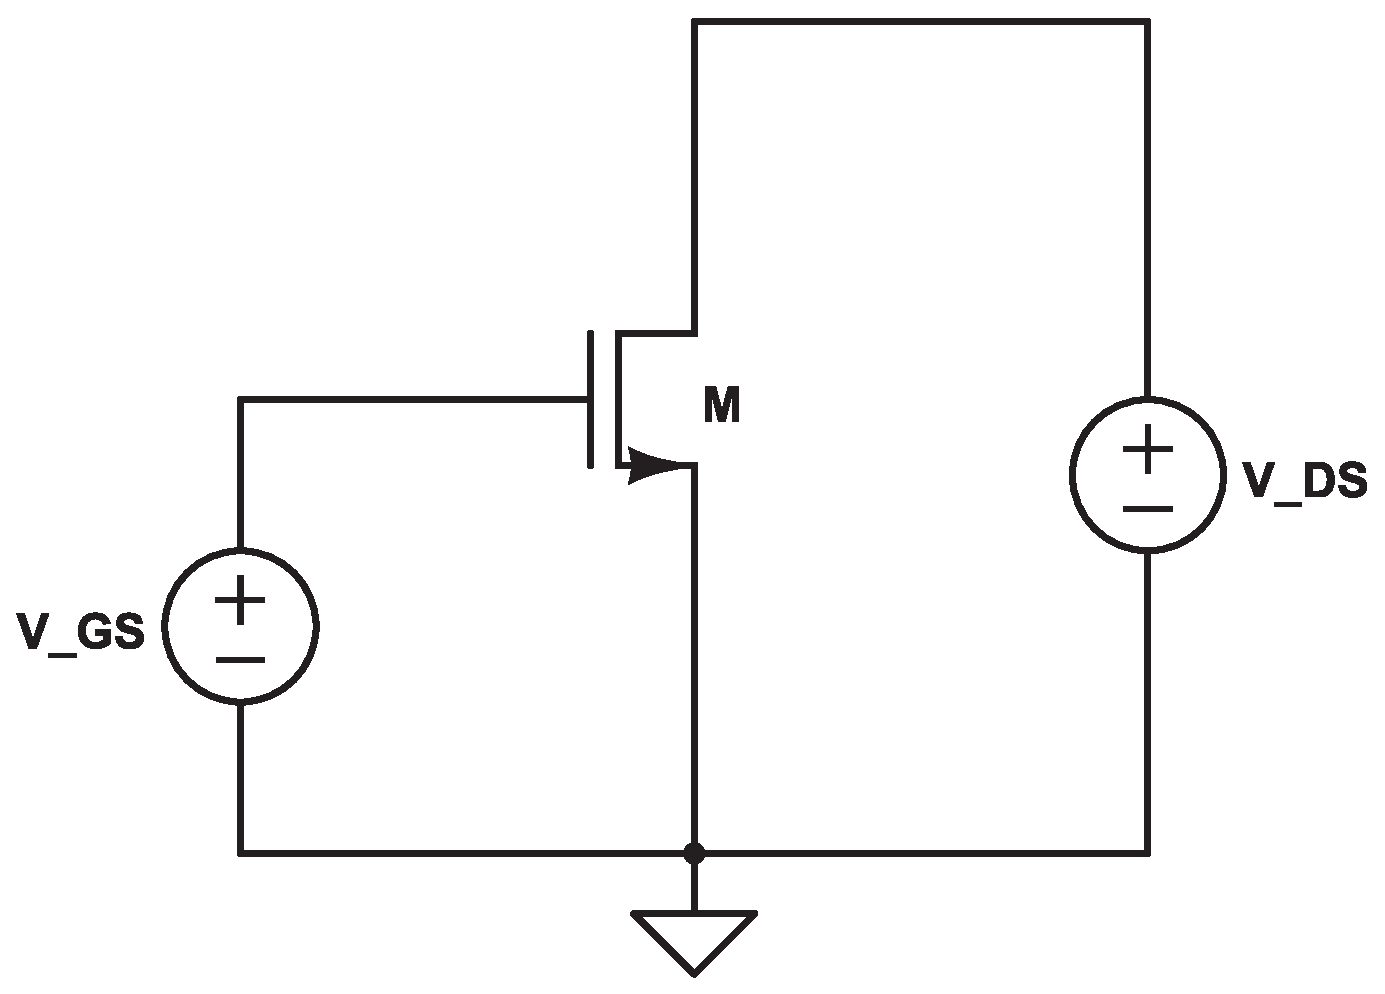
\includegraphics[width=0.5\textwidth]{resource/sim-circuit}
	\caption{Het circuit zoals gebruikt bij simulatie met SPICE}
	\label{fig:ump-sim-circuit}
\end{figure}

In dit circuit geldt als randvoorwaarde dat $V_{SB} = 0$, waaruit volgt dat $V_{T} = V_{T0}$ (zie sectie~\ref{sec:ump-theorie}).
Aan de hand van dit circuit kan vervolgens gesimuleerd worden met SPICE. Voor relevante simulatieresultaten kan als eerste een DC-sweep voor $I_{D}$ met als sweepvariabele $V_{DS}$ en tweede parameter $V_{GS}$ worden uitgevoerd. In figuur~\ref{fig:ump-sim-fig-vds} is het resultaat hiervan weergegeven. De grafiek is geplot met Matlab, het gebruikte script is te vinden in bijlage~\ref{lst:ump-plotVdsId}.
	
\begin{figure}[H]
	\centering
	\setlength\figureheight{0.4\textwidth} 
	\setlength\figurewidth{0.6\textwidth}
	% This file was created by matlab2tikz v0.4.2.
% Copyright (c) 2008--2013, Nico Schlömer <nico.schloemer@gmail.com>
% All rights reserved.
% 
% The latest updates can be retrieved from
%   http://www.mathworks.com/matlabcentral/fileexchange/22022-matlab2tikz
% where you can also make suggestions and rate matlab2tikz.
% 
% 
% 
%
% defining custom colors
\definecolor{mycolor1}{rgb}{0.8,1,0}%
\definecolor{mycolor2}{rgb}{0,1,0.4}%
\definecolor{mycolor3}{rgb}{0,0.4,1}%
\definecolor{mycolor4}{rgb}{0.800000000000001,0,1}%
\definecolor{mycolor5}{rgb}{0.75,0.75,0}%
%
\begin{tikzpicture}

\begin{axis}[%
width=\figurewidth,
height=\figureheight,
scale only axis,
xmin=0,
xmax=6.99999999999998,
xlabel={$V_{DS}$},
ymin=0,
ymax=0.00657962635159492,
ylabel={$I_{D}$},
axis x line*=bottom,
axis y line*=left,
legend style={draw=black,fill=white,legend cell align=left}
]
\addplot [
color=red,
solid
]
table[row sep=crcr]{
0 0\\
0.05 2.63460588030284e-05\\
0.1 4.82380200992338e-05\\
0.15 6.57152995700017e-05\\
0.2 7.88139586802572e-05\\
0.25 8.75671539688483e-05\\
0.3 9.18564983294345e-05\\
0.35 9.37392032938078e-05\\
0.4 9.52351838350296e-05\\
0.45 9.65605140663683e-05\\
0.5 9.77818344836123e-05\\
0.55 9.89303589449264e-05\\
0.6 0.000100023768027313\\
0.65 0.000101073288533371\\
0.7 0.000102086603874341\\
0.75 0.000103069243778009\\
0.8 0.000104025413747877\\
0.85 0.000104958351585083\\
0.9 0.00010587066935841\\
0.95 0.000106764484371524\\
1 0.000107641564682126\\
1.05 0.000108503387309611\\
1.1 0.000109351232822519\\
1.15 0.000110186192614492\\
1.2 0.000111009227111936\\
1.25 0.000111821180325933\\
1.3 0.000112622787128203\\
1.35 0.000113414724182803\\
1.4 0.000114197580842301\\
1.45 0.000114971902803518\\
1.5 0.000115738177555613\\
1.55 0.000116496841656044\\
1.6 0.000117248309834395\\
1.65 0.000117992953164503\\
1.7 0.000118731113616377\\
1.75 0.000119463111332152\\
1.8 0.000120189237350132\\
1.85 0.000120909768156707\\
1.9 0.000121624958410393\\
1.95 0.000122335040941834\\
2 0.000123040226753801\\
2.05 0.000123740755952895\\
2.1 0.000124436788610183\\
2.15 0.000125128528452478\\
2.2 0.000125816150102764\\
2.25 0.000126499799080193\\
2.3 0.000127179650007747\\
2.35 0.000127855833852664\\
2.4 0.00012852851068601\\
2.45 0.000129197767819278\\
2.5 0.00012986377987545\\
2.55 0.000130526634166017\\
2.6 0.000131186461658217\\
2.65 0.000131843349663541\\
2.7 0.00013249741459731\\
2.75 0.000133148758322932\\
2.8 0.000133797468151897\\
2.85 0.000134443631395698\\
2.9 0.000135087335365824\\
2.95 0.000135728667373769\\
3 0.000136367700179107\\
3.05 0.000137004521093331\\
3.1 0.000137639188324101\\
3.15 0.000138271774630994\\
3.2 0.0001389023673255\\
3.25 0.000139531010063365\\
3.3 0.000140157761052251\\
3.35 0.000140782693051733\\
3.4 0.000141405878821388\\
3.45 0.000142027347465046\\
3.5 0.000142647157190368\\
3.55 0.000143265366205014\\
3.6 0.000143882032716647\\
3.65 0.000144497200381011\\
3.69999999999999 0.000145110912853852\\
3.74999999999999 0.000145723228342831\\
3.79999999999999 0.000146334161399864\\
3.84999999999999 0.000146943799336441\\
3.89999999999999 0.000147552142152563\\
3.94999999999999 0.000148159262607805\\
3.99999999999999 0.000148765175254084\\
4.04999999999999 0.000149369923747145\\
4.09999999999999 0.000149973566294648\\
4.14999999999999 0.000150576117448509\\
4.19999999999999 0.000151177620864473\\
4.24999999999999 0.000151778105646372\\
4.29999999999999 0.00015237761544995\\
4.34999999999999 0.000152976164827123\\
4.39999999999999 0.000153573797433637\\
4.44999999999999 0.000154170542373322\\
4.49999999999999 0.000154766443301924\\
4.54999999999999 0.000155361500219442\\
4.59999999999999 0.000155955756781623\\
4.64999999999999 0.000156549242092296\\
4.69999999999999 0.000157141985255294\\
4.74999999999999 0.000157734015374444\\
4.79999999999999 0.000158325347001664\\
4.84999999999999 0.000158916009240784\\
4.89999999999999 0.000159506031195633\\
4.94999999999999 0.000160095441970043\\
4.99999999999999 0.000160684241564013\\
5.04999999999999 0.000161272473633289\\
5.09999999999999 0.000161860167281702\\
5.14999999999999 0.000162447322509252\\
5.19999999999999 0.000163033968419768\\
5.24999999999999 0.000163620134117082\\
5.29999999999999 0.000164205834153108\\
5.34999999999999 0.000164791097631678\\
5.39999999999999 0.000165375939104706\\
5.44999999999999 0.000165960358572192\\
5.49999999999999 0.000166544399689883\\
5.54999999999999 0.000167128077009693\\
5.59999999999999 0.000167711405083537\\
5.64999999999999 0.000168294413015246\\
5.69999999999999 0.000168877086252905\\
5.74999999999999 0.000169459483004175\\
5.79999999999999 0.00017004158871714\\
5.84999999999999 0.000170623432495631\\
5.89999999999999 0.000171205043443479\\
5.94999999999999 0.000171786407008767\\
5.99999999999999 0.000172367581399158\\
6.04999999999999 0.00017294853751082\\
6.09999999999999 0.000173529318999499\\
6.14999999999999 0.000174109925865196\\
6.19999999999999 0.00017469038721174\\
6.24999999999999 0.000175270703039132\\
6.29999999999999 0.000175850902451202\\
6.34999999999999 0.000176430999999866\\
6.39999999999999 0.000177010995685123\\
6.44999999999999 0.000177590904058889\\
6.49999999999998 0.000178170739673078\\
6.54999999999998 0.000178750531631522\\
6.59999999999998 0.000179330265382305\\
6.64999999999998 0.000179909984581172\\
6.69999999999998 0.000180489689228125\\
6.74999999999998 0.000181069379323162\\
6.79999999999998 0.000181649083970115\\
6.84999999999998 0.000182228803168982\\
6.89999999999998 0.000182808566023596\\
6.94999999999998 0.000183388357982039\\
6.99999999999998 0.000183968208148144\\
};
\addlegendentry{$V_{GS}: 1 V$};

\addplot [
color=mycolor1,
solid
]
table[row sep=crcr]{
0 0\\
0.05 7.49292084947228e-05\\
0.1 0.000146480320836417\\
0.15 0.000214678308111615\\
0.2 0.000279545987723395\\
0.25 0.000341104430845007\\
0.3 0.000399373035179451\\
0.35 0.000454369815997779\\
0.4 0.000506111595313996\\
0.45 0.000554614001885057\\
0.5 0.000599891762249172\\
0.55 0.000641958671621978\\
0.6 0.00068082771031186\\
0.65 0.000716511101927608\\
0.7 0.000749020429793745\\
0.75 0.000778366753365844\\
0.8 0.000802196154836565\\
0.85 0.000814971455838531\\
0.9 0.000824656221084297\\
0.95 0.000832951162010431\\
1 0.000840405293274671\\
1.05 0.000847279618028551\\
1.1 0.000853722391184419\\
1.15 0.00085982761811465\\
1.2 0.000865659210830927\\
1.25 0.00087126309517771\\
1.3 0.000876673555467278\\
1.35 0.000881917017977685\\
1.4 0.000887014379259199\\
1.45 0.000891982461325824\\
1.5 0.000896835117600858\\
1.55 0.000901583873201162\\
1.6 0.000906238507013768\\
1.65 0.000910807284526527\\
1.7 0.000915297481697053\\
1.75 0.000919715210329741\\
1.8 0.000924066000152379\\
1.85 0.000928354682400823\\
1.9 0.000932585564441979\\
1.95 0.000936762487981468\\
2 0.000940888829063624\\
2.05 0.000944967789109796\\
2.1 0.000949002045672387\\
2.15 0.000952994276303798\\
2.2 0.000956946809310466\\
2.25 0.000960861740168184\\
2.3 0.000964741047937423\\
2.35 0.000968586537055671\\
2.4 0.000972399895545095\\
2.45 0.00097618269501254\\
2.5 0.000979936448857188\\
2.55 0.000983662321232259\\
2.6 0.000987361650913954\\
2.65 0.000991035718470812\\
2.7 0.000994685455225408\\
2.75 0.000998312025330961\\
2.8 0.00100191636011004\\
2.85 0.00100549927446991\\
2.9 0.00100906181614846\\
2.95 0.00101260468363762\\
3 0.00101612857542932\\
3.05 0.00101963430643082\\
3.1 0.00102312269154936\\
3.15 0.00102659419644624\\
3.2 0.00103004940319806\\
3.25 0.00103348912671208\\
3.3 0.00103691383264959\\
3.35 0.00104032398667187\\
3.4 0.00104372017085552\\
3.45 0.00104710285086185\\
3.5 0.00105047249235213\\
3.55 0.00105382956098765\\
3.6 0.0010571745224297\\
3.65 0.00106050784233958\\
3.69999999999999 0.00106382975354791\\
3.74999999999999 0.00106714060530066\\
3.79999999999999 0.00107044097967446\\
3.84999999999999 0.00107373122591525\\
3.89999999999999 0.00107701146043837\\
3.94999999999999 0.0010802821489051\\
3.99999999999999 0.00108354352414608\\
4.04999999999999 0.0010867960518226\\
4.09999999999999 0.00109003984834999\\
4.14999999999999 0.0010932752629742\\
4.19999999999999 0.00109650264494121\\
4.24999999999999 0.00109972211066633\\
4.29999999999999 0.00110293400939554\\
4.34999999999999 0.00110613857395947\\
4.39999999999999 0.00110933603718877\\
4.44999999999999 0.00111252663191408\\
4.49999999999999 0.00111571059096605\\
4.54999999999999 0.00111888803075999\\
4.59999999999999 0.00112205930054188\\
4.64999999999999 0.00112522463314235\\
4.69999999999999 0.00112838402856141\\
4.74999999999999 0.00113153783604503\\
4.79999999999999 0.00113468628842384\\
4.84999999999999 0.00113782938569784\\
4.89999999999999 0.00114096736069769\\
4.94999999999999 0.00114410056266934\\
4.99999999999999 0.00114722887519747\\
5.04999999999999 0.00115035276394337\\
5.09999999999999 0.00115347211249173\\
5.14999999999999 0.00115658715367317\\
5.19999999999999 0.00115969812031835\\
5.24999999999999 0.00116280512884259\\
5.29999999999999 0.00116590841207653\\
5.34999999999999 0.00116900785360485\\
5.39999999999999 0.00117210380267352\\
5.44999999999999 0.00117519625928253\\
5.49999999999999 0.00117828557267785\\
5.54999999999999 0.00118137162644416\\
5.59999999999999 0.0011844546534121\\
5.64999999999999 0.001187534769997\\
5.69999999999999 0.00119061197619885\\
5.74999999999999 0.00119368662126362\\
5.79999999999999 0.00119675870519131\\
5.84999999999999 0.00119982822798193\\
5.89999999999999 0.00120289553888142\\
5.94999999999999 0.00120596052147448\\
5.99999999999999 0.00120902329217643\\
6.04999999999999 0.00121208420023322\\
6.09999999999999 0.00121514301281422\\
6.14999999999999 0.0012182000791654\\
6.19999999999999 0.00122125528287143\\
6.24999999999999 0.00122430897317827\\
6.29999999999999 0.0012273610336706\\
6.34999999999999 0.00123041158076376\\
6.39999999999999 0.00123346084728837\\
6.44999999999999 0.00123650871682912\\
6.49999999999998 0.00123955542221665\\
6.54999999999998 0.00124260107986629\\
6.59999999999998 0.00124564557336271\\
6.64999999999998 0.00124868925195187\\
6.69999999999998 0.00125173188280314\\
6.74999999999998 0.00125477381516248\\
6.79999999999998 0.00125781504902989\\
6.84999999999998 0.00126085558440536\\
6.89999999999998 0.00126389553770423\\
6.94999999999998 0.00126693502534181\\
6.99999999999998 0.00126997416373342\\
};
\addlegendentry{$V_{GS}: 2 V$};

\addplot [
color=mycolor2,
solid
]
table[row sep=crcr]{
0 0\\
0.05 0.000115335518785287\\
0.1 0.000227671131142415\\
0.15 0.000337028264766559\\
0.2 0.000443426542915404\\
0.25 0.000546884024515748\\
0.3 0.000647417444270104\\
0.35 0.000745042169000953\\
0.4 0.000839772750623524\\
0.45 0.000931622460484505\\
0.5 0.00102060404606164\\
0.55 0.00110672926530242\\
0.6 0.00119000929407775\\
0.65 0.0012704546097666\\
0.7 0.00134807522408664\\
0.75 0.00142288045026362\\
0.8 0.00149487913586199\\
0.85 0.0015640800120309\\
0.9 0.00163049099501222\\
0.95 0.00169411988463253\\
1 0.00175497401505709\\
1.05 0.00181306048762053\\
1.1 0.00186838593799621\\
1.15 0.00190638634376228\\
1.2 0.00193048210348934\\
1.25 0.00195011962205172\\
1.3 0.00196732394397259\\
1.35 0.00198293710127473\\
1.4 0.00199740473181009\\
1.45 0.00201099738478661\\
1.5 0.00202389364130795\\
1.55 0.00203621829859912\\
1.6 0.00204806355759501\\
1.65 0.00205949880182743\\
1.7 0.00207057851366699\\
1.75 0.00208134623244405\\
1.8 0.00209183688275516\\
1.85 0.00210208026692271\\
1.9 0.002112100366503\\
1.95 0.00212191813625395\\
2 0.00213155150413513\\
2.05 0.00214101560413837\\
2.1 0.00215032417327166\\
2.15 0.00215948885306716\\
2.2 0.00216851988807321\\
2.25 0.00217742659151554\\
2.3 0.00218621757812798\\
2.35 0.00219490006566048\\
2.4 0.0022034808062017\\
2.45 0.00221196585334837\\
2.5 0.00222036056220531\\
2.55 0.00222867052070796\\
2.6 0.00223689991980791\\
2.65 0.00224505318328738\\
2.7 0.00225313426926732\\
2.75 0.00226114667020738\\
2.8 0.00226909387856722\\
2.85 0.00227697915397584\\
2.9 0.00228480505757034\\
2.95 0.00229257461614907\\
3 0.00230029015801847\\
3.05 0.00230795424431562\\
3.1 0.00231556897051632\\
3.15 0.00232313643209636\\
3.2 0.00233065849170089\\
3.25 0.00233813747763634\\
3.3 0.00234557455405593\\
3.35 0.00235297158360481\\
3.4 0.00236033019609749\\
3.45 0.00236765202134848\\
3.5 0.00237493822351098\\
3.55 0.00238219019956887\\
3.6 0.002389409346506\\
3.65 0.00239659659564495\\
3.69999999999999 0.00240375334396958\\
3.74999999999999 0.00241088075563312\\
3.79999999999999 0.00241797952912748\\
3.84999999999999 0.00242505106143653\\
3.89999999999999 0.00243209628388286\\
3.94999999999999 0.00243911589495838\\
3.99999999999999 0.00244611082598567\\
4.04999999999999 0.00245308177545667\\
4.09999999999999 0.00246003014035523\\
4.14999999999999 0.00246695592068136\\
4.19999999999999 0.00247386051341891\\
4.24999999999999 0.00248074438422918\\
4.29999999999999 0.0024876082316041\\
4.34999999999999 0.00249445252120495\\
4.39999999999999 0.00250127818435431\\
4.44999999999999 0.0025080859195441\\
4.49999999999999 0.00251487595960498\\
4.54999999999999 0.00252164923585951\\
4.59999999999999 0.00252840598113835\\
4.64999999999999 0.00253514689393342\\
4.69999999999999 0.00254187267273664\\
4.74999999999999 0.00254858355037868\\
4.79999999999999 0.00255528022535145\\
4.84999999999999 0.00256196293048561\\
4.89999999999999 0.00256863236427307\\
4.94999999999999 0.00257528899237514\\
4.99999999999999 0.0025819328147918\\
5.04999999999999 0.00258856476284564\\
5.09999999999999 0.00259518506936729\\
5.14999999999999 0.0026017939671874\\
5.19999999999999 0.00260839215479791\\
5.24999999999999 0.00261497963219881\\
5.29999999999999 0.00262155709788203\\
5.34999999999999 0.00262812478467822\\
5.39999999999999 0.00263468292541802\\
5.44999999999999 0.00264123198576272\\
5.49999999999999 0.00264777219854295\\
5.54999999999999 0.00265430402942002\\
5.59999999999999 0.00266082747839391\\
5.64999999999999 0.00266734324395657\\
5.69999999999999 0.00267385132610798\\
5.74999999999999 0.00268035219050944\\
5.79999999999999 0.00268684606999159\\
5.84999999999999 0.00269333319738507\\
5.89999999999999 0.00269981380552053\\
5.94999999999999 0.00270628836005926\\
5.99999999999999 0.00271275686100125\\
6.04999999999999 0.00271921954117715\\
6.09999999999999 0.00272567686624825\\
6.14999999999999 0.00273212883621454\\
6.19999999999999 0.00273857591673732\\
6.24999999999999 0.00274501834064722\\
6.29999999999999 0.00275145610794425\\
6.34999999999999 0.00275788945145905\\
6.39999999999999 0.00276431883685291\\
6.44999999999999 0.00277074426412582\\
6.49999999999998 0.00277716619893909\\
6.54999999999998 0.00278358440846205\\
6.59999999999998 0.002789999358356\\
6.64999999999998 0.00279641128145158\\
6.69999999999998 0.0028028201777488\\
6.74999999999998 0.00280922651290894\\
6.79999999999998 0.00281563028693199\\
6.84999999999998 0.00282203149981797\\
6.89999999999998 0.00282843085005879\\
6.94999999999998 0.00283482787199318\\
6.99999999999998 0.00284122326411307\\
};
\addlegendentry{$V_{GS}: 3 V$};

\addplot [
color=mycolor3,
solid
]
table[row sep=crcr]{
0 0\\
0.05 0.000152013642946258\\
0.1 0.000301248859614134\\
0.15 0.000447725178673863\\
0.2 0.000591460557188839\\
0.25 0.000732471467927098\\
0.3 0.000870773161295801\\
0.35 0.00100637972354889\\
0.4 0.00113930436782539\\
0.45 0.00126955937594175\\
0.5 0.00139715615659952\\
0.55 0.00152210565283895\\
0.6 0.0016444178763777\\
0.65 0.0017641024896875\\
0.7 0.00188116845674813\\
0.75 0.00199562450870872\\
0.8 0.00210747867822647\\
0.85 0.00221673888154328\\
0.9 0.00232341233640909\\
0.95 0.00242750602774322\\
1 0.00252902670763433\\
1.05 0.00262798089534044\\
1.1 0.00272437487728894\\
1.15 0.00281821400858462\\
1.2 0.00290950457565486\\
1.25 0.00299825146794319\\
1.3 0.00308446027338505\\
1.35 0.00316523713991046\\
1.4 0.00321417511440814\\
1.45 0.00325011112727225\\
1.5 0.00328038237057626\\
1.55 0.00330727314576507\\
1.6 0.00333185330964625\\
1.65 0.00335472635924816\\
1.7 0.00337627273984253\\
1.75 0.00339674996212125\\
1.8 0.00341634219512343\\
1.85 0.00343518680892885\\
1.9 0.00345338857732713\\
1.95 0.00347103085368872\\
2 0.00348818046040833\\
2.05 0.00350489164702594\\
2.1 0.00352121028117836\\
2.15 0.00353717454709113\\
2.2 0.00355281657539308\\
2.25 0.00356816477142274\\
2.3 0.00358324334956706\\
2.35 0.00359807349741459\\
2.4 0.00361267384141684\\
2.45 0.0036270609125495\\
2.5 0.00364124937914312\\
2.55 0.00365525274537504\\
2.6 0.00366908241994679\\
2.65 0.00368274957872927\\
2.7 0.00369626353494823\\
2.75 0.00370963360182941\\
2.8 0.00372286746278405\\
2.85 0.0037359728012234\\
2.9 0.00374895636923611\\
2.95 0.00376182445324957\\
3 0.00377458287402987\\
3.05 0.00378723698668182\\
3.1 0.00379979168064892\\
3.15 0.00381225207820535\\
3.2 0.00382462213747203\\
3.25 0.00383690581656992\\
3.3 0.00384910730645061\\
3.35 0.00386123009957373\\
3.4 0.00387327745556831\\
3.45 0.00388525240123272\\
3.5 0.00389715796336532\\
3.55 0.00390899740159512\\
3.6 0.00392077257856727\\
3.65 0.00393248675391078\\
3.69999999999999 0.00394414179027081\\
3.74999999999999 0.00395574001595378\\
3.79999999999999 0.00396728422492743\\
3.84999999999999 0.00397877534851432\\
3.89999999999999 0.00399021664634347\\
3.94999999999999 0.00400160858407617\\
3.99999999999999 0.00401295395568013\\
4.04999999999999 0.00402425415813923\\
4.09999999999999 0.00403551058843732\\
4.14999999999999 0.00404672464355826\\
4.19999999999999 0.0040578986518085\\
4.24999999999999 0.00406903307884932\\
4.29999999999999 0.00408012978732586\\
4.34999999999999 0.00409119017422199\\
4.39999999999999 0.00410221517086029\\
4.44999999999999 0.00411320570856333\\
4.49999999999999 0.00412416364997625\\
4.54999999999999 0.00413508992642164\\
4.59999999999999 0.00414598546922207\\
4.64999999999999 0.00415685074403882\\
4.69999999999999 0.00416768807917833\\
4.74999999999999 0.00417849700897932\\
4.79999999999999 0.00418927939608693\\
4.84999999999999 0.00420003570616245\\
4.89999999999999 0.00421076687052846\\
4.94999999999999 0.00422147428616881\\
4.99999999999999 0.00423215795308352\\
5.04999999999999 0.00424281880259514\\
5.09999999999999 0.00425345776602626\\
5.14999999999999 0.00426407577469945\\
5.19999999999999 0.004274673294276\\
5.24999999999999 0.00428525079041719\\
5.29999999999999 0.00429580919444561\\
5.34999999999999 0.00430634943768382\\
5.39999999999999 0.00431687198579311\\
5.44999999999999 0.00432737683877349\\
5.49999999999999 0.00433786539360881\\
5.54999999999999 0.00434833765029907\\
5.59999999999999 0.00435879500582814\\
5.64999999999999 0.00436923699453473\\
5.69999999999999 0.00437966454774141\\
5.74999999999999 0.00439007859677076\\
5.79999999999999 0.00440047914162278\\
5.84999999999999 0.00441086664795876\\
5.89999999999999 0.00442124158143997\\
5.94999999999999 0.00443160487338901\\
5.99999999999999 0.00444195698946714\\
6.04999999999999 0.0044522974640131\\
6.09999999999999 0.00446262769401073\\
6.14999999999999 0.00447294814512134\\
6.19999999999999 0.00448325835168362\\
6.24999999999999 0.00449355924502015\\
6.29999999999999 0.00450385129079223\\
6.34999999999999 0.00451413495466113\\
6.39999999999999 0.00452441023662686\\
6.44999999999999 0.00453467760235071\\
6.49999999999998 0.00454493798315525\\
6.54999999999998 0.00455519091337919\\
6.59999999999998 0.00456543732434511\\
6.64999999999998 0.00457567721605301\\
6.69999999999998 0.00458591105416417\\
6.74999999999998 0.00459613930433989\\
6.79999999999998 0.00460636196658015\\
6.84999999999998 0.00461657950654626\\
6.89999999999998 0.00462679238989949\\
6.94999999999998 0.00463700061663985\\
6.99999999999998 0.00464720465242863\\
};
\addlegendentry{$V_{GS}: 4 V$};

\addplot [
color=mycolor4,
solid
]
table[row sep=crcr]{
0 0\\
0.05 0.000186325123650022\\
0.1 0.000370025110896677\\
0.15 0.000551118282601237\\
0.2 0.000729621504433453\\
0.25 0.000905550143215805\\
0.3 0.00107891857624054\\
0.35 0.00124974001664668\\
0.4 0.00141802674625069\\
0.45 0.00158379029016942\\
0.5 0.0017470414750278\\
0.55 0.00190779031254351\\
0.6 0.00206604646518826\\
0.65 0.00222181878052652\\
0.7 0.00237511587329209\\
0.75 0.00252594565972686\\
0.8 0.00267431582324207\\
0.85 0.00282023381441832\\
0.9 0.00296370615251362\\
0.95 0.00310473958961666\\
1 0.00324334064498544\\
1.05 0.00337951490655541\\
1.1 0.00351326842792332\\
1.15 0.00364460679702461\\
1.2 0.00377353490330279\\
1.25 0.00390005833469331\\
1.3 0.00402418151497841\\
1.35 0.00414590956643224\\
1.4 0.00426524644717574\\
1.45 0.00438219727948308\\
1.5 0.00449676578864455\\
1.55 0.00458967918530107\\
1.6 0.00464787520468235\\
1.65 0.00469437940046191\\
1.7 0.00473469868302345\\
1.75 0.00477103190496564\\
1.8 0.00480452459305525\\
1.85 0.00483586173504591\\
1.9 0.0048654917627573\\
1.95 0.00489372760057449\\
2 0.00492079742252827\\
2.05 0.0049468744546175\\
2.1 0.00497209234163165\\
2.15 0.00499655865132809\\
2.2 0.00502035999670625\\
2.25 0.00504356762394309\\
2.3 0.00506624253466725\\
2.35 0.00508843408897519\\
2.4 0.0051101865246892\\
2.45 0.00513153662905097\\
2.5 0.00515251746401191\\
2.55 0.00517315790057182\\
2.6 0.00519348215311766\\
2.65 0.00521351350471377\\
2.7 0.00523327151313424\\
2.75 0.00525277433916926\\
2.8 0.00527203781530261\\
2.85 0.00529107730835676\\
2.9 0.00530990492552519\\
2.95 0.00532853370532393\\
3 0.0053469748236239\\
3.05 0.00536523805931211\\
3.1 0.00538333272561431\\
3.15 0.00540126767009497\\
3.2 0.00541905080899596\\
3.25 0.00543668959289789\\
3.3 0.00545419100672007\\
3.35 0.00547156156972051\\
3.4 0.00548880686983466\\
3.45 0.00550593296065927\\
3.5 0.00552294496446848\\
3.55 0.00553984753787518\\
3.6 0.00555664580315351\\
3.65 0.00557334395125508\\
3.69999999999999 0.00558994570747018\\
3.74999999999999 0.00560645572841167\\
3.79999999999999 0.00562287727370858\\
3.84999999999999 0.00563921360298991\\
3.89999999999999 0.00565546797588468\\
3.94999999999999 0.00567164411768317\\
3.99999999999999 0.00568774482235312\\
4.04999999999999 0.00570377241820097\\
4.09999999999999 0.00571973016485572\\
4.14999999999999 0.00573562039062381\\
4.19999999999999 0.00575144542381167\\
4.24999999999999 0.00576720805838704\\
4.29999999999999 0.00578291015699506\\
4.34999999999999 0.00579855358228087\\
4.39999999999999 0.00581414112821221\\
4.44999999999999 0.00582967419177294\\
4.49999999999999 0.00584515510126948\\
4.54999999999999 0.00586058478802443\\
4.59999999999999 0.00587596604600549\\
4.64999999999999 0.00589130027219653\\
4.69999999999999 0.00590658839792013\\
4.74999999999999 0.00592183275148273\\
4.79999999999999 0.00593703472986817\\
4.84999999999999 0.00595219526439905\\
4.89999999999999 0.00596731575205922\\
4.94999999999999 0.00598239805549383\\
4.99999999999999 0.00599744357168674\\
5.04999999999999 0.00601245276629925\\
5.09999999999999 0.00602742750197649\\
5.14999999999999 0.00604236824437976\\
5.19999999999999 0.0060572768561542\\
5.24999999999999 0.0060721542686224\\
5.29999999999999 0.00608700141310692\\
5.34999999999999 0.00610181922093034\\
5.39999999999999 0.00611660862341523\\
5.44999999999999 0.00613137055188417\\
5.49999999999999 0.00614610640332103\\
5.54999999999999 0.00616081664338708\\
5.59999999999999 0.0061755022034049\\
5.64999999999999 0.00619016401469707\\
5.69999999999999 0.00620480300858617\\
5.74999999999999 0.00621941965073347\\
5.79999999999999 0.00623401533812284\\
5.84999999999999 0.00624859007075429\\
5.89999999999999 0.00626314524561167\\
5.94999999999999 0.00627768132835627\\
5.99999999999999 0.00629219878464937\\
6.04999999999999 0.00630669854581356\\
6.09999999999999 0.00632118107751012\\
6.14999999999999 0.00633564731106162\\
6.19999999999999 0.00635009817779064\\
6.24999999999999 0.00636453321203589\\
6.29999999999999 0.00637895427644253\\
6.34999999999999 0.00639336090534925\\
6.39999999999999 0.00640775449573994\\
6.44999999999999 0.00642213504761457\\
6.49999999999998 0.00643650349229574\\
6.54999999999998 0.00645086029544473\\
6.59999999999998 0.00646520592272282\\
6.64999999999998 0.00647954037413001\\
6.69999999999998 0.00649386504665017\\
6.74999999999998 0.0065081799402833\\
6.79999999999998 0.00652248598635197\\
6.84999999999998 0.00653678271919489\\
6.89999999999998 0.00655107153579593\\
6.94999999999998 0.00656535243615508\\
6.99999999999998 0.00657962635159492\\
};
\addlegendentry{$V_{GS}: 5 V$};

\addplot [
color=mycolor5,
solid
]
table[row sep=crcr]{
0 0\\
0.05 5.12573363084812e-06\\
0.1 2.05029345233925e-05\\
0.15 4.6131602677633e-05\\
0.2 8.20117380935699e-05\\
0.25 0.000128143340771203\\
0.3 0.000184526410710532\\
0.35 0.000251160947911558\\
0.4 0.000328046952374279\\
0.45 0.000415184424098697\\
0.5 0.000512573363084812\\
0.55 0.000620213769332622\\
0.6 0.000738105642842129\\
0.65 0.000866248983613332\\
0.7 0.00100464379164623\\
0.75 0.00115329006694083\\
0.8 0.00131218780949712\\
0.85 0.00148133701931511\\
0.9 0.00166073769639479\\
0.95 0.00185038984073617\\
1 0.00205029345233925\\
1.05 0.00226044853120402\\
1.1 0.00248085507733049\\
1.15 0.00271151309071865\\
1.2 0.00295242257136851\\
1.25 0.00320358351928007\\
1.3 0.00346499593445333\\
1.35 0.00373665981688828\\
1.4 0.00401857516658492\\
1.45 0.00431074198354326\\
1.5 0.0046131602677633\\
1.55 0.00492583001924504\\
1.6 0.00524875123798847\\
1.65 0.0055819239239936\\
1.7 0.00592534807726042\\
1.75 0.00627902369778894\\
1.8 0.00664295078557916\\
1.85 0.00701712934063107\\
1.9 0.00740155936294468\\
1.95 0.00779624085251998\\
2 0.00820117380935699\\
2.05 0.00861635823345568\\
2.1 0.00904179412481608\\
2.15 0.00947748148343817\\
2.2 0.00992342030932195\\
2.25 0.0103796106024674\\
2.3 0.0108460523628746\\
2.35 0.0113227455905435\\
2.4 0.0118096902854741\\
2.45 0.0123068864476663\\
2.5 0.0128143340771203\\
2.55 0.0133320331738359\\
2.6 0.0138599837378133\\
2.65 0.0143981857690524\\
2.7 0.0149466392675531\\
2.75 0.0155053442333156\\
2.8 0.0160743006663397\\
2.85 0.0166535085666255\\
2.9 0.0172429679341731\\
2.95 0.0178426787689823\\
3 0.0184526410710532\\
3.05 0.0190728548403858\\
3.1 0.0197033200769802\\
3.15 0.0203440367808362\\
3.2 0.0209950049519539\\
3.25 0.0216562245903333\\
3.3 0.0223276956959744\\
3.35 0.0230094182688772\\
3.4 0.0237013923090417\\
3.45 0.0244036178164679\\
3.5 0.0251160947911558\\
3.55 0.0258388232331053\\
3.6 0.0265718031423166\\
3.65 0.0273150345187896\\
3.69999999999999 0.0280685173625241\\
3.74999999999999 0.0288322516735205\\
3.79999999999999 0.0296062374517786\\
3.84999999999999 0.0303904746972983\\
3.89999999999999 0.0311849634100798\\
3.94999999999999 0.0319897035901229\\
3.99999999999999 0.0328046952374278\\
4.04999999999999 0.0336299383519943\\
4.09999999999999 0.0344654329338226\\
4.14999999999999 0.0353111789829125\\
4.19999999999999 0.0361671764992641\\
4.24999999999999 0.0370334254828775\\
4.29999999999999 0.0379099259337525\\
4.34999999999999 0.0387966778518892\\
4.39999999999999 0.0396936812372876\\
4.44999999999999 0.0406009360899477\\
4.49999999999999 0.0415184424098696\\
4.54999999999999 0.0424462001970531\\
4.59999999999999 0.0433842094514983\\
4.64999999999999 0.0443324701732052\\
4.69999999999999 0.0452909823621738\\
4.74999999999999 0.0462597460184041\\
4.79999999999999 0.047238761141896\\
4.84999999999999 0.0482280277326497\\
4.89999999999999 0.0492275457906651\\
4.94999999999999 0.0502373153159422\\
4.99999999999999 0.051257336308481\\
5.04999999999999 0.0522876087682814\\
5.09999999999999 0.0533281326953436\\
5.14999999999999 0.0543789080896674\\
5.19999999999999 0.055439934951253\\
5.24999999999999 0.0565112132801003\\
5.29999999999999 0.0575927430762092\\
5.34999999999999 0.0586845243395799\\
5.39999999999999 0.0597865570702122\\
5.44999999999999 0.0608988412681062\\
5.49999999999999 0.062021376933262\\
5.54999999999999 0.0631541640656794\\
5.59999999999999 0.0642972026653585\\
5.64999999999999 0.0654504927322993\\
5.69999999999999 0.0666140342665019\\
5.74999999999999 0.0677878272679661\\
5.79999999999999 0.068971871736692\\
5.84999999999999 0.0701661676726796\\
5.89999999999999 0.0713707150759289\\
5.94999999999999 0.0725855139464399\\
5.99999999999999 0.0738105642842126\\
6.04999999999999 0.075045866089247\\
6.09999999999999 0.0762914193615431\\
6.14999999999999 0.0775472241011009\\
6.19999999999999 0.0788132803079204\\
6.24999999999999 0.0800895879820016\\
6.29999999999999 0.0813761471233444\\
6.34999999999999 0.082672957731949\\
6.39999999999999 0.0839800198078152\\
6.44999999999999 0.0852973333509433\\
6.49999999999998 0.0866248983613326\\
6.54999999999998 0.087962714838984\\
6.59999999999998 0.089310782783897\\
6.64999999999998 0.0906691021960718\\
6.69999999999998 0.0920376730755082\\
6.74999999999998 0.0934164954222063\\
6.79999999999998 0.0948055692361662\\
6.84999999999998 0.0962048945173877\\
6.89999999999998 0.0976144712658709\\
6.94999999999998 0.0990342994816159\\
6.99999999999998 0.100464379164622\\
};
\addlegendentry{$V_{DS} \approx V_{GS} - V_{T}$};

\end{axis}
\end{tikzpicture}%
	\caption{SPICE-simulatie: $I_{D}$ uitgezet tegen $V_{DS}$ met vijf verschillende waarden voor $V_{GS}$. De lijn $V_{DS} \approx V_{GS} - V_{T}$ is een gefitte parabool en dient dus slechts als indicatie.}
	\label{fig:ump-sim-fig-vds}
\end{figure}

Uit deze simulatie kan de belangrijkste informatie worden gehaald om de vereiste parameters te bepalen, aan de hand van vergelijking~\ref{eq:ump-cmos-model-rab}. Vervolgens kan een aantal relevante datapunten in een tabel gezet worden, voor gebruik in vergelijking vergelijking~\ref{eq:ump-cmos-model-rab}, zie hiervoor tabel~\ref{tab:ump-sim-tab-vds}. De werkgebieden per datapunten zijn aannames, gemaakt aan de hand van figuur~\ref{fig:ump-sim-fig-vds}. Een daadwerkelijke waarde voor bijvoorbeeld $V_{DSAT}$ moet immers nog bepaald worden. De gebruikte waarden zijn zo bepaald, dat het uiteindelijke $V_{DS}$ - $I_{D}$-diagram de SPICE-simulatie zo dicht mogelijk benadert (enige fitting is dus nodig geweest).

\begin{table}[H]
	\centering
	\caption{Relevante waarden uit de simulatie van figuur \ref{fig:ump-sim-fig-vds}}
	\label{tab:ump-sim-tab-vds}
	\begin{tabular}{|c|c|c|c|c|} 	
		\hline
		Datapunt & $V_{GS}$ & $V_{DS}$ & $I_{D}$ & Werkgebied \\
		\hline
		1 & 1.2 V & 2.2 V & 0.2438 mA & Verzadiging \\
		\hline
		2 & 1.2 V & 2.6 V & 0.2292 mA & Verzadiging \\
		\hline
		3 & 1.4 V & 2.6 V & 0.3682 mA & Verzadiging \\
		\hline
		4 & 5.0 V & 5.0 V & 5.997 mA & Snelheidsverzadiging \\
		\hline	
	\end{tabular}
\end{table}

Daarnaast kan ook een DC-sweep voor $I_{D}$ met als sweepvariabele $V_{GS}$ en als tweede parameter $V_{DS}$ worden uitgevoerd. De resultaten van deze simulatie is te vinden in figuur~\ref{fig:ump-sim-fig-vgs}. Ook deze grafiek is geplot met Matlab, het gebruikte script is te vinden in bijlage~\ref{lst:ump-plotVgsId}.

\begin{figure}[H]
	\centering
	\setlength\figureheight{0.4\textwidth} 
	\setlength\figurewidth{0.6\textwidth}
	% This file was created by matlab2tikz v0.4.2.
% Copyright (c) 2008--2013, Nico Schlömer <nico.schloemer@gmail.com>
% All rights reserved.
% 
% The latest updates can be retrieved from
%   http://www.mathworks.com/matlabcentral/fileexchange/22022-matlab2tikz
% where you can also make suggestions and rate matlab2tikz.
% 
% 
% 
%
% defining custom colors
\definecolor{mycolor1}{rgb}{0.8,1,0}%
\definecolor{mycolor2}{rgb}{0,1,0.4}%
\definecolor{mycolor3}{rgb}{0,0.4,1}%
\definecolor{mycolor4}{rgb}{0.800000000000001,0,1}%
%
\begin{tikzpicture}

\begin{axis}[%
width=\figurewidth,
height=\figureheight,
scale only axis,
xmin=0,
xmax=5,
xlabel={$\text{V}_{\text{DS}}$},
ymin=0,
ymax=0.006,
ylabel={$\text{I}_{\text{D}}$},
axis x line*=bottom,
axis y line*=left,
legend style={draw=black,fill=white,legend cell align=left}
]
\addplot [
color=red,
solid
]
table[row sep=crcr]{
0 1.0100000263219e-12\\
0.05 1.0100000263219e-12\\
0.1 1.0100000263219e-12\\
0.15 1.0100000263219e-12\\
0.2 1.0100000263219e-12\\
0.25 1.0100000263219e-12\\
0.3 1.0100000263219e-12\\
0.35 1.0100000263219e-12\\
0.4 1.0100000263219e-12\\
0.45 1.0100000263219e-12\\
0.5 1.0100000263219e-12\\
0.55 1.0100000263219e-12\\
0.6 1.5014289544979e-07\\
0.65 3.16215050588653e-06\\
0.7 1.00194811238907e-05\\
0.75 2.06770528166089e-05\\
0.8 3.38614954671357e-05\\
0.85 4.90048551000655e-05\\
0.9 6.64367325953208e-05\\
0.95 8.6021980678197e-05\\
1 0.000107641564682126\\
1.05 0.000131187989609316\\
1.1 0.000156562600750476\\
1.15 0.000183673648280092\\
1.2 0.000212435144931078\\
1.25 0.000242765905568376\\
1.3 0.000274588936008513\\
1.35 0.000307830836391076\\
1.4 0.000342421553796157\\
1.45 0.000378293887479231\\
1.5 0.000415383226936683\\
1.55 0.000453627435490489\\
1.6 0.000492966442834586\\
1.65 0.000533342128619552\\
1.7 0.0005746980314143\\
1.75 0.000616979144979268\\
1.8 0.000660131685435772\\
1.85 0.000704102742020041\\
1.9 0.000748840102460235\\
1.95 0.000794291670899838\\
2 0.000840405293274671\\
2.05 0.000887127942405641\\
2.1 0.000934405135922134\\
2.15 0.000982180004939437\\
2.2 0.00103039166424423\\
2.25 0.00107897387351841\\
2.3 0.00112785154487938\\
2.35 0.00117693655192852\\
2.4 0.00122611946426332\\
2.45 0.001275256392546\\
2.5 0.00132413930259645\\
2.55 0.00137242884375155\\
2.6 0.00141944875940681\\
2.65 0.00146349414717406\\
2.7 0.00150597305037081\\
2.75 0.00154815602581948\\
2.8 0.00159005343448371\\
2.85 0.0016316749388352\\
2.9 0.00167302985209972\\
2.95 0.00171412678901106\\
3 0.00175497401505709\\
3.05 0.00179557933006436\\
3.1 0.0018359498353675\\
3.15 0.00187609274871647\\
3.2 0.0019160145893693\\
3.25 0.00195572152733803\\
3.3 0.00199521984905005\\
3.35 0.00203451467677951\\
3.4 0.00207361206412315\\
3.45 0.00211251666769385\\
3.5 0.00215123360976577\\
3.55 0.00218976777978241\\
3.6 0.00222812336869538\\
3.65 0.00226630480028689\\
3.69999999999999 0.00230431626550853\\
3.74999999999999 0.00234216172248125\\
3.79999999999999 0.00237984512932599\\
3.84999999999999 0.00241736974567175\\
3.89999999999999 0.00245473929680884\\
3.94999999999999 0.00249195727519691\\
3.99999999999999 0.00252902670763433\\
4.04999999999999 0.00256595085375011\\
4.09999999999999 0.00260273274034262\\
4.14999999999999 0.00263937516137958\\
4.19999999999999 0.00267588091082871\\
4.24999999999999 0.00271225278265774\\
4.29999999999999 0.00274849310517311\\
4.34999999999999 0.00278460490517318\\
4.39999999999999 0.00282059004530311\\
4.44999999999999 0.00285645131953061\\
4.49999999999999 0.00289219082333148\\
4.54999999999999 0.00292781088501215\\
4.59999999999999 0.00296331336721778\\
4.64999999999999 0.00299870036542416\\
4.69999999999999 0.00303397420793772\\
4.74999999999999 0.00306913652457297\\
4.79999999999999 0.0031041894108057\\
4.84999999999999 0.00313913426361978\\
4.89999999999999 0.00317397341132164\\
4.94999999999999 0.00320870825089514\\
4.99999999999999 0.00324334064498544\\
};
\addlegendentry{$\text{V}_{\text{DS}}\text{: 1 V}$};

\addplot [
color=mycolor1,
solid
]
table[row sep=crcr]{
0 2.0100000223261e-12\\
0.05 2.0100000223261e-12\\
0.1 2.0100000223261e-12\\
0.15 2.0100000223261e-12\\
0.2 2.0100000223261e-12\\
0.25 2.0100000223261e-12\\
0.3 2.0100000223261e-12\\
0.35 2.0100000223261e-12\\
0.4 2.0100000223261e-12\\
0.45 2.0100000223261e-12\\
0.5 2.0100000223261e-12\\
0.55 2.0100000223261e-12\\
0.6 6.21847959791921e-07\\
0.65 4.97702603752259e-06\\
0.7 1.34689662445453e-05\\
0.75 2.60522465396207e-05\\
0.8 4.06464750994928e-05\\
0.85 5.76944912609179e-05\\
0.9 7.71966952015646e-05\\
0.95 9.90182961686514e-05\\
1 0.000123040226753801\\
1.05 0.000149154991959222\\
1.1 0.000177263966179453\\
1.15 0.000207275690627284\\
1.2 0.000239104687352665\\
1.25 0.000272670586127788\\
1.3 0.000307897542370483\\
1.35 0.000344713684171438\\
1.4 0.000383050821255893\\
1.45 0.000422844052081928\\
1.5 0.000464031647425145\\
1.55 0.00050655473023653\\
1.6 0.000550357217434794\\
1.65 0.000595385557971895\\
1.7 0.00064158852910623\\
1.75 0.000688917411025614\\
1.8 0.000737325521185994\\
1.85 0.000786768330726773\\
1.9 0.000837203289847821\\
1.95 0.000888589769601822\\
2 0.000940888829063624\\
2.05 0.000994063448160887\\
2.1 0.00104807794559747\\
2.15 0.0011028986191377\\
2.2 0.00115849287249148\\
2.25 0.00121482962276787\\
2.3 0.00127187941689044\\
2.35 0.00132961373310536\\
2.4 0.00138800556305796\\
2.45 0.00144702871330082\\
2.5 0.00150665850378573\\
2.55 0.0015668710693717\\
2.6 0.00162764359265566\\
2.65 0.00168895442038774\\
2.7 0.00175078259781003\\
2.75 0.00181310810148716\\
2.8 0.00187591172289103\\
2.85 0.00193917518481612\\
2.9 0.00200288067571819\\
2.95 0.00206701154820621\\
3 0.00213155150413513\\
3.05 0.00219648494385183\\
3.1 0.00226179673336446\\
3.15 0.00232747290283442\\
3.2 0.00239349971525371\\
3.25 0.00245986343361437\\
3.3 0.00252655171789229\\
3.35 0.00259355246089399\\
3.4 0.002660853555426\\
3.45 0.00272844405844808\\
3.5 0.00279631279408932\\
3.55 0.00286444928497076\\
3.6 0.00293284351937473\\
3.65 0.00300148595124483\\
3.69999999999999 0.00307036680169404\\
3.74999999999999 0.00313947745598853\\
3.79999999999999 0.00320880906656384\\
3.84999999999999 0.00327835301868618\\
3.89999999999999 0.00334810162894428\\
3.94999999999999 0.00341804651543498\\
3.99999999999999 0.00348818046040833\\
4.04999999999999 0.00355849601328373\\
4.09999999999999 0.00362898618914187\\
4.14999999999999 0.00369964400306344\\
4.19999999999999 0.00377046316862106\\
4.24999999999999 0.00384143693372607\\
4.29999999999999 0.00391255924478173\\
4.34999999999999 0.00398382358253002\\
4.39999999999999 0.00405522529035807\\
4.44999999999999 0.00412675738334656\\
4.49999999999999 0.00419841520488262\\
4.54999999999999 0.0042701936326921\\
4.59999999999999 0.00434208661317825\\
4.64999999999999 0.0044140899553895\\
4.69999999999999 0.00448619807139039\\
4.74999999999999 0.00455840677022934\\
4.79999999999999 0.00463071092963219\\
4.84999999999999 0.00470310635864735\\
4.89999999999999 0.00477558886632323\\
4.94999999999999 0.00484815379604697\\
4.99999999999999 0.00492079742252827\\
};
\addlegendentry{$\text{V}_{\text{DS}}\text{: 2 V}$};

\addplot [
color=mycolor2,
solid
]
table[row sep=crcr]{
0 3.01000001833029e-12\\
0.05 3.01000001833029e-12\\
0.1 3.01000001833029e-12\\
0.15 3.01000001833029e-12\\
0.2 3.01000001833029e-12\\
0.25 3.01000001833029e-12\\
0.3 3.01000001833029e-12\\
0.35 3.01000001833029e-12\\
0.4 3.01000001833029e-12\\
0.45 3.01000001833029e-12\\
0.5 3.01000001833029e-12\\
0.55 3.01000001833029e-12\\
0.6 1.25803285300208e-06\\
0.65 6.79662207403453e-06\\
0.7 1.6720594430808e-05\\
0.75 3.07796326524112e-05\\
0.8 4.67087447759695e-05\\
0.85 6.53814859106205e-05\\
0.9 8.66380214574747e-05\\
0.95 0.000110340784885921\\
1 0.000136367700179107\\
1.05 0.000164608150953427\\
1.1 0.000194960433873348\\
1.15 0.000227330092457123\\
1.2 0.000261628738371655\\
1.25 0.000297773163765669\\
1.3 0.000335684831952676\\
1.35 0.000375289237126708\\
1.4 0.000416515686083585\\
1.45 0.000459296890767291\\
1.5 0.000503568851854652\\
1.55 0.000549270422197878\\
1.6 0.000596343481447548\\
1.65 0.000644732324872166\\
1.7 0.000694383983500302\\
1.75 0.0007452477584593\\
1.8 0.000797275279182941\\
1.85 0.000850420328788459\\
1.9 0.000904638669453561\\
1.95 0.000959888217039406\\
2 0.00101612857542932\\
2.05 0.00107332121115178\\
2.1 0.00113142933696508\\
2.15 0.00119041767902672\\
2.2 0.00125025259330869\\
2.25 0.00131090194918215\\
2.3 0.00137233489658684\\
2.35 0.00143452209886163\\
2.4 0.00149743538349867\\
2.45 0.00156104774214327\\
2.5 0.00162533356342465\\
2.55 0.00169026805087924\\
2.6 0.00175582768861204\\
2.65 0.00182198989205062\\
2.7 0.00188873300794512\\
2.75 0.00195603631436825\\
2.8 0.00202388013713062\\
2.85 0.00209224526770413\\
2.9 0.00216111354529858\\
2.95 0.00223046727478504\\
3 0.00230029015801847\\
3.05 0.00237056612968445\\
3.1 0.00244127935729921\\
3.15 0.0025124151725322\\
3.2 0.00258395983837545\\
3.25 0.00265589915215969\\
3.3 0.00272822030819952\\
3.35 0.00280091096647084\\
3.4 0.00287395855411887\\
3.45 0.00294735189527273\\
3.5 0.00302107958123088\\
3.55 0.00309513113461435\\
3.6 0.00316949607804418\\
3.65 0.00324416439980268\\
3.69999999999999 0.00331912678666413\\
3.74999999999999 0.0033943741582334\\
3.79999999999999 0.00346989720128477\\
3.84999999999999 0.00354568753391504\\
3.89999999999999 0.00362173723988235\\
3.94999999999999 0.00369803817011416\\
3.99999999999999 0.00377458287402987\\
4.04999999999999 0.00385136366821826\\
4.09999999999999 0.00392837356775999\\
4.14999999999999 0.0040056062862277\\
4.19999999999999 0.00408305460587144\\
4.24999999999999 0.00416071200743318\\
4.29999999999999 0.00423857290297747\\
4.34999999999999 0.00431663123890758\\
4.39999999999999 0.00439488096162677\\
4.44999999999999 0.0044733164831996\\
4.49999999999999 0.00455193314701319\\
4.54999999999999 0.00463072489947081\\
4.59999999999999 0.00470968708395958\\
4.64999999999999 0.00478881550952792\\
4.69999999999999 0.0048681041225791\\
4.74999999999999 0.0049475496634841\\
4.79999999999999 0.00502714747563004\\
4.84999999999999 0.00510689243674278\\
4.89999999999999 0.00518678175285459\\
4.94999999999999 0.00526681030169129\\
4.99999999999999 0.0053469748236239\\
};
\addlegendentry{$\text{V}_{\text{DS}}\text{: 3 V}$};

\addplot [
color=mycolor3,
solid
]
table[row sep=crcr]{
0 4.00999979749406e-12\\
0.05 4.00999979749406e-12\\
0.1 4.00999979749406e-12\\
0.15 4.00999979749406e-12\\
0.2 4.00999979749406e-12\\
0.25 4.00999979749406e-12\\
0.3 4.00999979749406e-12\\
0.35 4.00999979749406e-12\\
0.4 4.00999979749406e-12\\
0.45 4.00999979749406e-12\\
0.5 4.00999979749406e-12\\
0.55 4.00999979749406e-12\\
0.6 2.00291310648026e-06\\
0.65 8.64114190335386e-06\\
0.7 1.98946072487161e-05\\
0.75 3.51273811247665e-05\\
0.8 5.24327842867933e-05\\
0.85 7.26019279682077e-05\\
0.9 9.5471870736219e-05\\
0.95 0.00012090152449673\\
1 0.000148765175254084\\
1.05 0.00017894858319778\\
1.1 0.000211346516152844\\
1.15 0.000245861068833619\\
1.2 0.000282400549622253\\
1.25 0.000320878549246117\\
1.3 0.000361213402356952\\
1.35 0.000403327750973403\\
1.4 0.000447147962404415\\
1.45 0.00049260415835306\\
1.5 0.000539629545528442\\
1.55 0.000588160706683993\\
1.6 0.000638136931229383\\
1.65 0.000689500360749662\\
1.7 0.000742195814382285\\
1.75 0.000796170381363481\\
1.8 0.000851373770274222\\
1.85 0.00090775778517127\\
1.9 0.000965276383794844\\
1.95 0.00102388567756861\\
2 0.00108354352414608\\
2.05 0.00114420987665653\\
2.1 0.00120584631804377\\
2.15 0.00126841606106609\\
2.2 0.00133188418112695\\
2.25 0.00139621691778302\\
2.3 0.0014613822568208\\
2.35 0.00152734958101064\\
2.4 0.00159408955369145\\
2.45 0.00166157400235534\\
2.5 0.00172977591864765\\
2.55 0.00179866992402822\\
2.6 0.00186823098920286\\
2.65 0.0019384358311072\\
2.7 0.00200926186516881\\
2.75 0.00208068732172251\\
2.8 0.00215269136242568\\
2.85 0.00222525442950428\\
2.9 0.0022983574308455\\
2.95 0.00237198197282851\\
3 0.00244611082598567\\
3.05 0.00252072676084936\\
3.1 0.0025958139449358\\
3.15 0.00267135701142251\\
3.2 0.00274734105914831\\
3.25 0.00282375165261328\\
3.3 0.00290057552047074\\
3.35 0.00297779915854335\\
3.4 0.00305540999397635\\
3.45 0.00313339591957629\\
3.5 0.00321174506098032\\
3.55 0.00329044670797884\\
3.6 0.00336948968470097\\
3.65 0.00344886374659836\\
3.69999999999999 0.00352855864912272\\
3.74999999999999 0.00360856484621763\\
3.79999999999999 0.00368887325748801\\
3.84999999999999 0.00376947480253875\\
3.89999999999999 0.00385036109946668\\
3.94999999999999 0.00393152330070734\\
3.99999999999999 0.00401295395568013\\
4.04999999999999 0.00409464491531253\\
4.09999999999999 0.00417658919468522\\
4.14999999999999 0.00425877934321761\\
4.19999999999999 0.00434120837599039\\
4.24999999999999 0.00442386977374554\\
4.29999999999999 0.00450675701722503\\
4.34999999999999 0.00458986358717084\\
4.39999999999999 0.00467318389564753\\
4.44999999999999 0.00475671235471964\\
4.49999999999999 0.00484044244512916\\
4.54999999999999 0.00492436904460192\\
4.59999999999999 0.00500848703086376\\
4.64999999999999 0.00509279174730182\\
4.69999999999999 0.00517727760598063\\
4.74999999999999 0.00526193995028734\\
4.79999999999999 0.00534677458927035\\
4.84999999999999 0.00543177640065551\\
4.89999999999999 0.00551694165915251\\
4.94999999999999 0.00560226570814848\\
4.99999999999999 0.00568774482235312\\
};
\addlegendentry{$\text{V}_{\text{DS}}\text{: 4 V}$};

\addplot [
color=mycolor4,
solid
]
table[row sep=crcr]{
0 5.00999979349825e-12\\
0.05 5.00999979349825e-12\\
0.1 5.00999979349825e-12\\
0.15 5.00999979349825e-12\\
0.2 5.00999979349825e-12\\
0.25 5.00999979349825e-12\\
0.3 5.00999979349825e-12\\
0.35 5.00999979349825e-12\\
0.4 5.00999979349825e-12\\
0.45 5.00999979349825e-12\\
0.5 5.00999979349825e-12\\
0.55 1.44762148934774e-08\\
0.6 2.832834070432e-06\\
0.65 1.05232902569696e-05\\
0.7 2.30493133130949e-05\\
0.75 3.93691916542593e-05\\
0.8 5.79878396820277e-05\\
0.85 7.9585071944166e-05\\
0.9 0.000103994309029076\\
0.95 0.000131070570205338\\
1 0.000160684241564013\\
1.05 0.00019271727069281\\
1.1 0.000227060707402416\\
1.15 0.000263613095739856\\
1.2 0.000302279251627624\\
1.25 0.000342969520715997\\
1.3 0.000385599094443023\\
1.35 0.000430087500717491\\
1.4 0.00047635831288062\\
1.45 0.000524338742252439\\
1.5 0.000573959550820291\\
1.55 0.000625154585577548\\
1.6 0.00067786080762744\\
1.65 0.000732018030248582\\
1.7 0.000787568744271994\\
1.75 0.000844458118081093\\
1.8 0.000902633706573397\\
1.85 0.000962045392952859\\
1.9 0.00102264527231455\\
1.95 0.00108438776805997\\
2 0.00114722887519747\\
2.05 0.00121112714987248\\
2.1 0.00127604231238365\\
2.15 0.00134193641133606\\
2.2 0.00140877289231867\\
2.25 0.00147651683073491\\
2.3 0.00154513469897211\\
2.35 0.0016145947156474\\
2.4 0.00168486626353115\\
2.45 0.00175592012237757\\
2.5 0.00182772835250944\\
2.55 0.00190026417840272\\
2.6 0.0019735018722713\\
2.65 0.00204741698689759\\
2.7 0.00212198588997126\\
2.75 0.00219718599691987\\
2.8 0.00227299612015486\\
2.85 0.00234939530491829\\
2.9 0.00242636352777481\\
2.95 0.00250388216227293\\
3 0.0025819328147918\\
3.05 0.00266049802303314\\
3.1 0.00273956102319062\\
3.15 0.00281910574994981\\
3.2 0.00289911637082696\\
3.25 0.00297957868315279\\
3.3 0.00306047778576612\\
3.35 0.00314180040732026\\
3.4 0.00322353304363787\\
3.45 0.00330566335469484\\
3.5 0.00338817900046706\\
3.55 0.00347106833942235\\
3.6 0.00355431996285915\\
3.65 0.00363792316056788\\
3.69999999999999 0.00372186745516956\\
3.74999999999999 0.00380614283494651\\
3.79999999999999 0.00389073928818107\\
3.84999999999999 0.00397564796730876\\
3.89999999999999 0.00406085979193449\\
3.94999999999999 0.0041463659144938\\
3.99999999999999 0.00423215795308352\\
4.04999999999999 0.00431822752580047\\
4.09999999999999 0.00440456764772534\\
4.14999999999999 0.00449117040261626\\
4.19999999999999 0.00457802880555391\\
4.24999999999999 0.0046651354059577\\
4.29999999999999 0.0047524836845696\\
4.34999999999999 0.00484006712213159\\
4.39999999999999 0.00492787919938564\\
4.44999999999999 0.00501591386273503\\
4.49999999999999 0.0051041659899056\\
4.54999999999999 0.00519262859597802\\
4.59999999999999 0.00528129749000072\\
4.64999999999999 0.00537016615271568\\
4.69999999999999 0.00545922992751002\\
4.74999999999999 0.00554848415777087\\
4.79999999999999 0.00563792372122407\\
4.84999999999999 0.00572754396125674\\
4.89999999999999 0.00581734022125602\\
4.94999999999999 0.00590730784460902\\
4.99999999999999 0.00599744357168674\\
};
\addlegendentry{$\text{V}_{\text{DS}}\text{: 5 V}$};

\end{axis}
\end{tikzpicture}%
	\caption{SPICE-simulatie: $I_{D}$ uitgezet tegen $V_{GS}$ met vijf verschillende waarden voor $V_{DS}$}
	\label{fig:ump-sim-fig-vgs}
\end{figure}

Dit figuur biedt een indicatie voor de threshholdspanning, $V_{T0}$. Te zien is dat de stroom pas bij een gate-sourcespanning ($V_GS$) van 0.7 V begint op te lopen. Bij de algebraïsche bepaling van een waarde voor $V_{T0}$ is deze 0.7 V dus een waarde om rekening mee te houden. Voor de verdere verwerking van de simulatieresultaten komt deze grafiek niet meer aan de orde en wordt alleen de data uit figuur~\ref{fig:ump-sim-fig-vds} gebruikt.
\\

Met bovenstaande data kunnen de gevraagde parameters vervolgens berekend worden.

\subsection{Verwerking}
\label{subsec:ump-methode-verw}
\subsubsection{Drempelspanning}
\label{subsubsec:ump-methode-verw-vt0}
Voor het berekenen van $V_{T0}$ gebruiken we vergelijking~\ref{eq:ump-cmos-model-rab} tweemaal voor twee verschillende datapunten in het verzadigingsgebied van de transistor, waarbij $V_{DS}$ constant is. De vergelijking voor de drainstroom is dan als volgt:

\begin{equation} \label{eq:ump-cmos-model-rab-sat}
	I_{D} = \frac{1}{2} k (V_{GS} - V_{T})^2(1 + \lambda V_{DS})
\end{equation}

Deze uitdrukking kan worden omgeschreven naar de volgende:

$$\frac{2}{k(1 + \lambda V_{DS)}} = \frac{(V_{GS} - V_{T})^2}{I_{D}}$$

Aangezien $V_{DS}$ over de twee datapunten constant gehouden is en $\lambda$ en $k$ transistoreigenschappen zijn die dus gedurende de gehele simulatie constant blijven, geldt het volgende voor de twee datapunten:

$$\frac{1}{k(1 + \lambda V_{DS1})} = \frac{1}{k(1 + \lambda V_{DS2})}$$

Dan mag gesteld worden dat:

$$\frac{(V_{GS1} - V_{T})^2}{I_{D1}} = \frac{(V_{GS2} - V_{T})^2}{I_{D2}} \Rightarrow I_{D1}(V_{GS2} - V_{T})^2 = I_{D2}(V_{GS1} - V_{T})^2$$

Waaruit een uitdrukking voor $V_{T}$ kan worden afgeleid, die afhankelijk is van twee waarden voor $V_{GS}$ en $I_{D}$ bij gelijke $V_{DS}$. En dus, omdat $V_{SB} = 0$ en dus $V_{T0} = V_{T}$ bereiken we de uiteindelijke uitdrukking voor $V_{T0}$:

\begin{equation} \label{eq:ump-vt0}
	V_{T0} = \frac{\sqrt{I_{D1}}V_{GS2} - \sqrt{I_{D2}}V_{GS1}}{\sqrt{I_{D1}} - \sqrt{I_{D2}}}
\end{equation}

\subsubsection{Lambda}
\label{subsubsec:ump-methode-verw-lambda}
Voor het berekenen van $\lambda$ kan min of meer dezelfde methode worden gebruikt als voor $V_{T0}$. Nu kiezen we echter twee datapunten waarop $V_{GS}$ constant is. Vergelijking~\ref{eq:ump-cmos-model-rab-sat} kan dan worden omgeschreven naar de volgende uitdrukking:

$$\frac{2}{k(V_{GS}-V_{T})^2} = \frac{1 + \lambda V_{DS}}{I_{D}}$$

Nu is $V_{GS}$ over de twee datapunten constant en zijn $k$ en $V_{T}$ constante transistoreigenschappen, dus geldt:

$$\frac{2}{k(V_{GS1}-V_{T})^2} = \frac{2}{k(V_{GS2}-V_{T})^2}$$

En ook:

$$\frac{1 + \lambda V_{DS1}}{I_{D1}} = \frac{1 + \lambda V_{DS2}}{I_{D2}} \Rightarrow I_{D2}(1 + \lambda V_{DS1}) = I_{D1}(1 + \lambda V_{DS2})$$

Waaruit dan de uiteindelijke vergelijking voor $\lambda$ kan worden afgeleid. Deze is dan afhankelijk van de twee verschillende waarden van $V_{DS}$ en $I_{D}$:

\begin{equation} \label{eq:ump-lambda}
	\lambda = \frac{I_{D1} - I_{D2}}{V_{DS1}I_{D2} - V_{DS2}I_{D1}}
\end{equation}

\subsubsection{k'}
\label{subsubsec:ump-methode-verw-kprime}
Met $V_{T}$ en $\lambda$ zijn twee van de drie onbekende parameters uit vergelijking~\ref{eq:ump-cmos-model-rab-sat} berekend, er blijft dus slechts één onbekende over. Deze kan vervolgens voor willekeurige waarden van $V_{DS}$ en $V_{GS}$ worden berekend, mits in het verzadigingsgebied. Uit vergelijking~\ref{eq:ump-cmos-model-rab-sat} volgt dan voor $k$:

$$k = \frac{2I_{D}}{(V_{GS} - V_{T})^2(1 + \lambda V_{DS})}$$

Dan volgt hieruit, omdat zoals al eerder vermeld geldt dat $k = k'\frac{W}{L}$, de uiteindelijke uitdrukking voor $k'$:

\begin{equation} \label{eq:ump-kprime}
	k' = \frac{L}{W}\frac{2I_{D}}{(V_{GS} - V_{T})^2(1 + \lambda V_{DS})}
\end{equation}

\subsubsection{Snelheidsverzadiging}
\label{subsubsec:ump-methode-verw-vdsat}
Omdat in het voorgaande elke onbekende uit het model van Rabaey is bepaald, kan deze opgelost worden voor $V_{DSAT}$, waarna alle reeds bepaalde parameters, samen met waarden voor $V_{DS}$, $V_{GS}$ en de bijbehorende waarde van $I_{D}$ kunnen worden ingevuld om tot een oplossing te komen. Een voorwaarde aan de waarde van $V_{DS}$ is uiteraard dat deze in het snelheidsverzadigingswerkgebied van de transistor valt. Het model van Rabaey geeft de volgende vergelijking voor $I_{D}$:

\begin{equation}
	I_{D} = k' \frac{W}{L}[(V_{GS} - V_{T})V_{DSAT} - \frac{V_{DSAT}^2}{2}](1 + \lambda V_{DS})
\end{equation}

Oplossen van deze vergelijking levert een tweedegraads vergelijking op:

$$-k'\frac{W}{2L}V_{DSAT}^2 + k'\frac{W}{L}(V_{GS}-V_{T})V_{DSAT} - \frac{I_{D}}{1 + \lambda V_{DS}} = 0$$

Met de wortelformule lost deze vergelijking op tot de uiteindelijke uitdrukking voor $V_{DSAT}$:

\begin{equation} \label{eq:ump-vdsat}
	V_{DSAT} = \frac{-k'\frac{W}{L}(V_{GS}-V_{T}) \pm \sqrt{[k'\frac{W}{L}(V_{GS}-V_{T})]^2 - k'\frac{2W}{L}\frac{I_{D}}{1 + \lambda V_{DS}}}}{-k'\frac{W}{L}}
\end{equation}

Met deze laatste uitdrukkingen is er voor iedere gevraagde parameter een uitdrukking.

\section{Resultaten}
\label{sec:ump-res}
\subsection{Waarden}
\label{subsec:ump-res-val}
Om waarden voor de vier gevraagde parameters te bepalen, vullen we de relevante waarden uit tabel~\ref{tab:ump-sim-tab-vds} in de vergelijkingen uit sectie~\ref{subsec:ump-methode-verw}.

\subsubsection{Drempelspanning}
\label{subsubsec:ump-res-val-vt0}
Ten eerste bepalen we $V_{T0}$. Hiervoor nemen we twee datapunten uit tabel~\ref{tab:ump-sim-tab-vds}, met gelijke $V_{DS}$, welke in het verzadigingsgebied valt. Dit zijn datapunten 2 en 3. Deze vullen we vervolgens in vergelijking \ref{eq:ump-vt0}. Dit geeft:

\begin{equation} \label{ump-vt0-num}
	V_{T0} = \frac{1.4\sqrt{0.2292 \cdot 10^{-3}} - 1.2\sqrt{0.3682 \cdot 10^{-3}}}{\sqrt{0.2292 \cdot 10^{-3}} - \sqrt{0.3682 \cdot 10^{-3}}} = 0.4521 \, \textrm{V}
\end{equation}

\subsubsection{Lambda}
\label{subsubsec:ump-res-val-lambda}
Vervolgens nemen we datapunten 1 en 2 om $\lambda$ te bepalen aan de hand van vergelijking~\ref{eq:ump-lambda}:

\begin{equation} \label{ump-lambda-num}
	\lambda = \frac{0.2438 \cdot 10^{-3} - 0.2292 \cdot 10^{-3}}{2.6 \cdot 0.2292 \cdot 10^{-3} - 2.2 \cdot 0.2438 \cdot 10^{-3}} = 0.1281 \, \textrm{V}^{-1}
\end{equation}

\subsubsection{k'}
\label{subsubsec:ump-res-val-kprime}
Dan kunnen de gegevens van datapunt 3 samen met de zojuist berekende $V_{T0}$ en $\lambda$ gebruikt worden in vergelijking~\ref{eq:ump-kprime} om $k'$ te berekenen:

\begin{equation} \label{eq:ump-kprime-num}
	k' = \frac{1.6 \cdot 10^{-6}}{23.2 \cdot 10^{-6}}\frac{2 \cdot 0.3682 \cdot 10^{-3}}{(1.4 - 0.4521)^2(1 + 0.1281 \cdot 2.6)} = 0.4690 \,\frac{\textrm{mA}}{\textrm{V}^{2}}
\end{equation}

\subsubsection{Snelheidsverzadiging}
\label{subsubsec:ump-res-val-vdsat}
Als laatste komen de gegevens van datapunt 4 met elke reeds berekende parameter samen om $V_{DSAT}$ te berekenen met vergelijking~\ref{eq:ump-vdsat}:

\begin{equation} \label{eq:ump-vdsat-num}
	V_{DSAT} = \frac{-46.90 \cdot 10^{-6}\frac{23.2 \cdot 10^{-6}}{1.6 \cdot 10^{-6}}(5-0.4521) \pm \sqrt{[46.90 \cdot 10^{-6}\frac{23.2 \cdot 10^{-6}}{1.6 \cdot 10^{-6}}(5-0.4521)]^2 - 46.90 \cdot 10^{-6}\frac{2 \cdot 23.2 \cdot 10^{-6}}{1.6 \cdot 10^{-6}}\frac{5.997 \cdot 10^{-3}}{1 + 0.1281 \cdot 5}}}{-46.90 \cdot 10^{-6}\frac{23.2 \cdot 10^{-6}}{1.6 \cdot 10^{-6}}}	
\end{equation}

$$V_{DSAT} = 1.396 \, \textrm{V} \vee V_{DSAT} = 7.700 \, \textrm{V}$$

Hierbij is 1.396 V een aannemelijke waarde, 7.700 V niet, deze ligt te hoog om normaal gedrag van de transistor te veroorzaken. Opvallend is, dat de gekozen waarde voor $V_{GS}$ (zie tabel~\ref{tab:ump-sim-tab-vds}, datapunt 3) nu iets boven $V_{DSAT}$ blijken te liggen, waardoor eigenlijk niet aan de randvoorwaarden wordt voldaan. Wanneer $V_{GS}$ echter lager werd gemaakt om toch onder deze waarde van $V_{DSAT}$ te blijven, daalde die gewoon mee. Wij hebben hier geen verklaring voor.

\subsection{Simulatie en vergelijking}
\label{sec:ump-res-verg}
Er zijn meteen een aantal opvallendheden aan de berekende parameters. Zo ligt $V_{T0}$ veel lager dan de verwachte 0.7 V en ook wanneer we de waarden vergelijken met de in de handleiding *gegeven parameters zijn er grote verschillen. Een vergelijk is gemaakt in tabel~\ref{tab:ump-par-comp}. Het SPICE-model lijkt alleen een waarde voor $V_{T0}$ te bevatten (eveneens 0.7 V) en is daarom niet opgenomen in de tabel. Daarnaast zijn de waarden die in het boek van Rabaey gegeven staan voor een transistor van een geheel andere orde van grootte dan die op de Sea-of-Gates-chip en daarom niet geheel relevant. \cite[103]{rabaey-integrated-circuits}

\begin{table}[H]
	\centering
	\caption{Een vergelijking tussen de berekende en gegeven waarden. \cite[98]{epo3-manual}}
	\label{tab:ump-par-comp}
	\begin{tabular}{|c|c|c|c|} 	
		\hline
		Parameter & Berekende waarde & Gegeven waarde & Relatieve afwijking \\
		\hline
		$V_{T0}$ & $0.4521 \,\textrm{V}$ & $0.7 \,\textrm{V}$ & $65\%$ \\
		\hline
		$\lambda$ & $0.1281 \,\textrm{V}^{-1}$ & $0.027 \,\textrm{V}^{-1}$ & $474\%$ \\
		\hline
		$k$ ($\beta$) & $0.4690 \,\frac{\textrm{mA}}{\textrm{V}^{2}}$ & $0.65 \,\frac{\textrm{mA}}{\textrm{V}^{2}}$ & $72\%$ \\
		\hline
		$V_{DSAT}$ & $1.396 \, \textrm{V}$ & - & - \\
		\hline	
	\end{tabular}
\end{table}

Er kan echter pas echt bepaald worden of de bepaalde parameters een goed model vormen voor het gedrag van de transistor aan de hand van een simulatie. Voor deze simulatie is een Matlab-script gemaakt, dat te vinden is in bijlage~\ref{lst-ump-simulate}. Het script rekent een set gegeven waarden, zoals in tabel~\ref{tab:ump-sim-tab-vds} om naar de correcte parameterwaarden, volgens de vergelijkingen uit sectie~\ref{subsec:ump-methode-verw} en plot deze vervolgens, samen met de simulatieresultaten uit SPICE. Onderstaande grafiek (figuur \ref{fig:ump-sim-fig-vds-rab}) is het resultaat met de parameters zoals berekend in sectie~\ref{subsec:ump-res-val}.

\begin{figure}[H]
	\centering
	\setlength\figureheight{0.4\textwidth} 
	\setlength\figurewidth{0.6\textwidth}
	% This file was created by matlab2tikz v0.4.2.
% Copyright (c) 2008--2013, Nico Schlömer <nico.schloemer@gmail.com>
% All rights reserved.
% 
% The latest updates can be retrieved from
%   http://www.mathworks.com/matlabcentral/fileexchange/22022-matlab2tikz
% where you can also make suggestions and rate matlab2tikz.
% 
% 
% 
%
% defining custom colors
\definecolor{mycolor1}{rgb}{0.846153846153846,1,0}%
\definecolor{mycolor2}{rgb}{0,1,0.307692307692308}%
\definecolor{mycolor3}{rgb}{0,0.538461538461539,1}%
\definecolor{mycolor4}{rgb}{0.615384615384616,0,1}%
\definecolor{mycolor5}{rgb}{1,0,0.230769230769231}%
%
\begin{tikzpicture}

\begin{axis}[%
width=\figurewidth,
height=\figureheight,
scale only axis,
xmin=0,
xmax=7,
xlabel={$V_{DS}$},
ymin=0,
ymax=0.00693408087593374,
ylabel={$I_{D}$},
axis x line*=bottom,
axis y line*=left,
legend style={draw=black,fill=white,legend cell align=left}
]
\addplot [
color=mycolor1,
solid
]
table[row sep=crcr]{
0 0\\
0.05 1.78954929981712e-05\\
0.1 3.42967370608792e-05\\
0.15 4.91710615344745e-05\\
0.2 6.24857957653074e-05\\
0.25 7.42082690997281e-05\\
0.3 8.43058108840869e-05\\
0.35 9.27457504647342e-05\\
0.4 9.94954171880202e-05\\
0.45 0.000104522140400295\\
0.5 0.00010779324944791\\
0.55 0.000109277662974423\\
0.6 0.000109931524494457\\
0.65 0.000110585386014491\\
0.7 0.000111239247534526\\
0.75 0.00011189310905456\\
0.8 0.000112546970574594\\
0.85 0.000113200832094628\\
0.9 0.000113854693614663\\
0.95 0.000114508555134697\\
1 0.000115162416654731\\
1.05 0.000115816278174766\\
1.1 0.0001164701396948\\
1.15 0.000117124001214834\\
1.2 0.000117777862734868\\
1.25 0.000118431724254903\\
1.3 0.000119085585774937\\
1.35 0.000119739447294971\\
1.4 0.000120393308815005\\
1.45 0.00012104717033504\\
1.5 0.000121701031855074\\
1.55 0.000122354893375108\\
1.6 0.000123008754895143\\
1.65 0.000123662616415177\\
1.7 0.000124316477935211\\
1.75 0.000124970339455245\\
1.8 0.00012562420097528\\
1.85 0.000126278062495314\\
1.9 0.000126931924015348\\
1.95 0.000127585785535383\\
2 0.000128239647055417\\
2.05 0.000128893508575451\\
2.1 0.000129547370095485\\
2.15 0.00013020123161552\\
2.2 0.000130855093135554\\
2.25 0.000131508954655588\\
2.3 0.000132162816175623\\
2.35 0.000132816677695657\\
2.4 0.000133470539215691\\
2.45 0.000134124400735725\\
2.5 0.00013477826225576\\
2.55 0.000135432123775794\\
2.6 0.000136085985295828\\
2.65 0.000136739846815863\\
2.7 0.000137393708335897\\
2.75 0.000138047569855931\\
2.8 0.000138701431375965\\
2.85 0.000139355292896\\
2.9 0.000140009154416034\\
2.95 0.000140663015936068\\
3 0.000141316877456103\\
3.05 0.000141970738976137\\
3.1 0.000142624600496171\\
3.15 0.000143278462016205\\
3.2 0.00014393232353624\\
3.25 0.000144586185056274\\
3.3 0.000145240046576308\\
3.35 0.000145893908096343\\
3.4 0.000146547769616377\\
3.45 0.000147201631136411\\
3.5 0.000147855492656445\\
3.55 0.00014850935417648\\
3.6 0.000149163215696514\\
3.65 0.000149817077216548\\
3.7 0.000150470938736582\\
3.75 0.000151124800256617\\
3.8 0.000151778661776651\\
3.85 0.000152432523296685\\
3.9 0.00015308638481672\\
3.95 0.000153740246336754\\
4 0.000154394107856788\\
4.05 0.000155047969376822\\
4.1 0.000155701830896857\\
4.15 0.000156355692416891\\
4.2 0.000157009553936925\\
4.25 0.00015766341545696\\
4.3 0.000158317276976994\\
4.35 0.000158971138497028\\
4.4 0.000159625000017062\\
4.45 0.000160278861537097\\
4.5 0.000160932723057131\\
4.55 0.000161586584577165\\
4.6 0.0001622404460972\\
4.65 0.000162894307617234\\
4.7 0.000163548169137268\\
4.75 0.000164202030657302\\
4.8 0.000164855892177337\\
4.85 0.000165509753697371\\
4.9 0.000166163615217405\\
4.95 0.00016681747673744\\
5 0.000167471338257474\\
5.05 0.000168125199777508\\
5.1 0.000168779061297542\\
5.15 0.000169432922817577\\
5.2 0.000170086784337611\\
5.25 0.000170740645857645\\
5.3 0.000171394507377679\\
5.35 0.000172048368897714\\
5.4 0.000172702230417748\\
5.45 0.000173356091937782\\
5.5 0.000174009953457817\\
5.55 0.000174663814977851\\
5.6 0.000175317676497885\\
5.65 0.000175971538017919\\
5.7 0.000176625399537954\\
5.75 0.000177279261057988\\
5.8 0.000177933122578022\\
5.85 0.000178586984098057\\
5.9 0.000179240845618091\\
5.95 0.000179894707138125\\
6 0.000180548568658159\\
6.05 0.000181202430178194\\
6.1 0.000181856291698228\\
6.15 0.000182510153218262\\
6.2 0.000183164014738297\\
6.25 0.000183817876258331\\
6.3 0.000184471737778365\\
6.35 0.000185125599298399\\
6.4 0.000185779460818434\\
6.45 0.000186433322338468\\
6.5 0.000187087183858502\\
6.55 0.000187741045378537\\
6.6 0.000188394906898571\\
6.65 0.000189048768418605\\
6.7 0.000189702629938639\\
6.75 0.000190356491458674\\
6.8 0.000191010352978708\\
6.85 0.000191664214498742\\
6.9 0.000192318076018777\\
6.95 0.000192971937538811\\
7 0.000193625799058845\\
};
\addlegendentry{$V_{GS}: 1 V$};

\addplot [
color=mycolor1,
dashed,
forget plot
]
table[row sep=crcr]{
0 0\\
0.05 2.63460588030284e-05\\
0.1 4.82380200992338e-05\\
0.15 6.57152995700017e-05\\
0.2 7.88139586802572e-05\\
0.25 8.75671539688483e-05\\
0.3 9.18564983294345e-05\\
0.35 9.37392032938078e-05\\
0.4 9.52351838350296e-05\\
0.45 9.65605140663683e-05\\
0.5 9.77818344836123e-05\\
0.55 9.89303589449264e-05\\
0.6 0.000100023768027313\\
0.65 0.000101073288533371\\
0.7 0.000102086603874341\\
0.75 0.000103069243778009\\
0.8 0.000104025413747877\\
0.85 0.000104958351585083\\
0.9 0.00010587066935841\\
0.95 0.000106764484371524\\
1 0.000107641564682126\\
1.05 0.000108503387309611\\
1.1 0.000109351232822519\\
1.15 0.000110186192614492\\
1.2 0.000111009227111936\\
1.25 0.000111821180325933\\
1.3 0.000112622787128203\\
1.35 0.000113414724182803\\
1.4 0.000114197580842301\\
1.45 0.000114971902803518\\
1.5 0.000115738177555613\\
1.55 0.000116496841656044\\
1.6 0.000117248309834395\\
1.65 0.000117992953164503\\
1.7 0.000118731113616377\\
1.75 0.000119463111332152\\
1.8 0.000120189237350132\\
1.85 0.000120909768156707\\
1.9 0.000121624958410393\\
1.95 0.000122335040941834\\
2 0.000123040226753801\\
2.05 0.000123740755952895\\
2.1 0.000124436788610183\\
2.15 0.000125128528452478\\
2.2 0.000125816150102764\\
2.25 0.000126499799080193\\
2.3 0.000127179650007747\\
2.35 0.000127855833852664\\
2.4 0.00012852851068601\\
2.45 0.000129197767819278\\
2.5 0.00012986377987545\\
2.55 0.000130526634166017\\
2.6 0.000131186461658217\\
2.65 0.000131843349663541\\
2.7 0.00013249741459731\\
2.75 0.000133148758322932\\
2.8 0.000133797468151897\\
2.85 0.000134443631395698\\
2.9 0.000135087335365824\\
2.95 0.000135728667373769\\
3 0.000136367700179107\\
3.05 0.000137004521093331\\
3.1 0.000137639188324101\\
3.15 0.000138271774630994\\
3.2 0.0001389023673255\\
3.25 0.000139531010063365\\
3.3 0.000140157761052251\\
3.35 0.000140782693051733\\
3.4 0.000141405878821388\\
3.45 0.000142027347465046\\
3.5 0.000142647157190368\\
3.55 0.000143265366205014\\
3.6 0.000143882032716647\\
3.65 0.000144497200381011\\
3.7 0.000145110912853852\\
3.75 0.000145723228342831\\
3.8 0.000146334161399864\\
3.85 0.000146943799336441\\
3.9 0.000147552142152563\\
3.95 0.000148159262607805\\
4 0.000148765175254084\\
4.05 0.000149369923747145\\
4.1 0.000149973566294648\\
4.15 0.000150576117448509\\
4.2 0.000151177620864473\\
4.25 0.000151778105646372\\
4.3 0.00015237761544995\\
4.35 0.000152976164827123\\
4.4 0.000153573797433637\\
4.45 0.000154170542373322\\
4.5 0.000154766443301924\\
4.55 0.000155361500219442\\
4.6 0.000155955756781623\\
4.65 0.000156549242092296\\
4.7 0.000157141985255294\\
4.75 0.000157734015374444\\
4.8 0.000158325347001664\\
4.85 0.000158916009240784\\
4.9 0.000159506031195633\\
4.95 0.000160095441970043\\
5 0.000160684241564013\\
5.05 0.000161272473633289\\
5.1 0.000161860167281702\\
5.15 0.000162447322509252\\
5.2 0.000163033968419768\\
5.25 0.000163620134117082\\
5.3 0.000164205834153108\\
5.35 0.000164791097631678\\
5.4 0.000165375939104706\\
5.45 0.000165960358572192\\
5.5 0.000166544399689883\\
5.55 0.000167128077009693\\
5.6 0.000167711405083537\\
5.65 0.000168294413015246\\
5.7 0.000168877086252905\\
5.75 0.000169459483004175\\
5.8 0.00017004158871714\\
5.85 0.000170623432495631\\
5.9 0.000171205043443479\\
5.95 0.000171786407008767\\
6 0.000172367581399158\\
6.05 0.00017294853751082\\
6.1 0.000173529318999499\\
6.15 0.000174109925865196\\
6.2 0.00017469038721174\\
6.25 0.000175270703039132\\
6.3 0.000175850902451202\\
6.35 0.000176430999999866\\
6.4 0.000177010995685123\\
6.45 0.000177590904058889\\
6.5 0.000178170739673078\\
6.55 0.000178750531631522\\
6.6 0.000179330265382305\\
6.65 0.000179909984581172\\
6.7 0.000180489689228125\\
6.75 0.000181069379323162\\
6.8 0.000181649083970115\\
6.85 0.000182228803168982\\
6.9 0.000182808566023596\\
6.95 0.000183388357982039\\
7 0.000183968208148144\\
};
\addplot [
color=mycolor2,
solid
]
table[row sep=crcr]{
0 0\\
0.05 5.21183546009396e-05\\
0.1 0.000103178068981745\\
0.15 0.000153146472488768\\
0.2 0.000201990894468357\\
0.25 0.000249678664266863\\
0.3 0.000296177111230636\\
0.35 0.000341453564706028\\
0.4 0.000385475354039387\\
0.45 0.000428209808577065\\
0.5 0.000469624257665411\\
0.55 0.000509686030650776\\
0.6 0.000548362456879511\\
0.65 0.000585620865697965\\
0.7 0.000621428586452488\\
0.75 0.000655752948489432\\
0.8 0.000688561281155147\\
0.85 0.000719820913795982\\
0.9 0.000749499175758288\\
0.95 0.000777563396388416\\
1 0.000803980905032715\\
1.05 0.000828719031037536\\
1.1 0.00085174510374923\\
1.15 0.000873026452514146\\
1.2 0.000892530406678635\\
1.25 0.000910224295589048\\
1.3 0.000926075448591733\\
1.35 0.000940051195033043\\
1.4 0.000951675595983955\\
1.45 0.000956844189304418\\
1.5 0.00096201278262488\\
1.55 0.000967181375945343\\
1.6 0.000972349969265805\\
1.65 0.000977518562586267\\
1.7 0.00098268715590673\\
1.75 0.000987855749227192\\
1.8 0.000993024342547654\\
1.85 0.000998192935868117\\
1.9 0.00100336152918858\\
1.95 0.00100853012250904\\
2 0.0010136987158295\\
2.05 0.00101886730914997\\
2.1 0.00102403590247043\\
2.15 0.00102920449579089\\
2.2 0.00103437308911135\\
2.25 0.00103954168243182\\
2.3 0.00104471027575228\\
2.35 0.00104987886907274\\
2.4 0.0010550474623932\\
2.45 0.00106021605571367\\
2.5 0.00106538464903413\\
2.55 0.00107055324235459\\
2.6 0.00107572183567505\\
2.65 0.00108089042899551\\
2.7 0.00108605902231598\\
2.75 0.00109122761563644\\
2.8 0.0010963962089569\\
2.85 0.00110156480227736\\
2.9 0.00110673339559783\\
2.95 0.00111190198891829\\
3 0.00111707058223875\\
3.05 0.00112223917555921\\
3.1 0.00112740776887968\\
3.15 0.00113257636220014\\
3.2 0.0011377449555206\\
3.25 0.00114291354884106\\
3.3 0.00114808214216153\\
3.35 0.00115325073548199\\
3.4 0.00115841932880245\\
3.45 0.00116358792212291\\
3.5 0.00116875651544337\\
3.55 0.00117392510876384\\
3.6 0.0011790937020843\\
3.65 0.00118426229540476\\
3.7 0.00118943088872522\\
3.75 0.00119459948204569\\
3.8 0.00119976807536615\\
3.85 0.00120493666868661\\
3.9 0.00121010526200707\\
3.95 0.00121527385532754\\
4 0.001220442448648\\
4.05 0.00122561104196846\\
4.1 0.00123077963528892\\
4.15 0.00123594822860939\\
4.2 0.00124111682192985\\
4.25 0.00124628541525031\\
4.3 0.00125145400857077\\
4.35 0.00125662260189123\\
4.4 0.0012617911952117\\
4.45 0.00126695978853216\\
4.5 0.00127212838185262\\
4.55 0.00127729697517308\\
4.6 0.00128246556849355\\
4.65 0.00128763416181401\\
4.7 0.00129280275513447\\
4.75 0.00129797134845493\\
4.8 0.0013031399417754\\
4.85 0.00130830853509586\\
4.9 0.00131347712841632\\
4.95 0.00131864572173678\\
5 0.00132381431505725\\
5.05 0.00132898290837771\\
5.1 0.00133415150169817\\
5.15 0.00133932009501863\\
5.2 0.0013444886883391\\
5.25 0.00134965728165956\\
5.3 0.00135482587498002\\
5.35 0.00135999446830048\\
5.4 0.00136516306162094\\
5.45 0.00137033165494141\\
5.5 0.00137550024826187\\
5.55 0.00138066884158233\\
5.6 0.00138583743490279\\
5.65 0.00139100602822326\\
5.7 0.00139617462154372\\
5.75 0.00140134321486418\\
5.8 0.00140651180818464\\
5.85 0.00141168040150511\\
5.9 0.00141684899482557\\
5.95 0.00142201758814603\\
6 0.00142718618146649\\
6.05 0.00143235477478696\\
6.1 0.00143752336810742\\
6.15 0.00144269196142788\\
6.2 0.00144786055474834\\
6.25 0.0014530291480688\\
6.3 0.00145819774138927\\
6.35 0.00146336633470973\\
6.4 0.00146853492803019\\
6.45 0.00147370352135065\\
6.5 0.00147887211467112\\
6.55 0.00148404070799158\\
6.6 0.00148920930131204\\
6.65 0.0014943778946325\\
6.7 0.00149954648795297\\
6.75 0.00150471508127343\\
6.8 0.00150988367459389\\
6.85 0.00151505226791435\\
6.9 0.00152022086123482\\
6.95 0.00152538945455528\\
7 0.00153055804787574\\
};
\addlegendentry{$V_{GS}: 2 V$};

\addplot [
color=mycolor2,
dashed,
forget plot
]
table[row sep=crcr]{
0 0\\
0.05 7.49292084947228e-05\\
0.1 0.000146480320836417\\
0.15 0.000214678308111615\\
0.2 0.000279545987723395\\
0.25 0.000341104430845007\\
0.3 0.000399373035179451\\
0.35 0.000454369815997779\\
0.4 0.000506111595313996\\
0.45 0.000554614001885057\\
0.5 0.000599891762249172\\
0.55 0.000641958671621978\\
0.6 0.00068082771031186\\
0.65 0.000716511101927608\\
0.7 0.000749020429793745\\
0.75 0.000778366753365844\\
0.8 0.000802196154836565\\
0.85 0.000814971455838531\\
0.9 0.000824656221084297\\
0.95 0.000832951162010431\\
1 0.000840405293274671\\
1.05 0.000847279618028551\\
1.1 0.000853722391184419\\
1.15 0.00085982761811465\\
1.2 0.000865659210830927\\
1.25 0.00087126309517771\\
1.3 0.000876673555467278\\
1.35 0.000881917017977685\\
1.4 0.000887014379259199\\
1.45 0.000891982461325824\\
1.5 0.000896835117600858\\
1.55 0.000901583873201162\\
1.6 0.000906238507013768\\
1.65 0.000910807284526527\\
1.7 0.000915297481697053\\
1.75 0.000919715210329741\\
1.8 0.000924066000152379\\
1.85 0.000928354682400823\\
1.9 0.000932585564441979\\
1.95 0.000936762487981468\\
2 0.000940888829063624\\
2.05 0.000944967789109796\\
2.1 0.000949002045672387\\
2.15 0.000952994276303798\\
2.2 0.000956946809310466\\
2.25 0.000960861740168184\\
2.3 0.000964741047937423\\
2.35 0.000968586537055671\\
2.4 0.000972399895545095\\
2.45 0.00097618269501254\\
2.5 0.000979936448857188\\
2.55 0.000983662321232259\\
2.6 0.000987361650913954\\
2.65 0.000991035718470812\\
2.7 0.000994685455225408\\
2.75 0.000998312025330961\\
2.8 0.00100191636011004\\
2.85 0.00100549927446991\\
2.9 0.00100906181614846\\
2.95 0.00101260468363762\\
3 0.00101612857542932\\
3.05 0.00101963430643082\\
3.1 0.00102312269154936\\
3.15 0.00102659419644624\\
3.2 0.00103004940319806\\
3.25 0.00103348912671208\\
3.3 0.00103691383264959\\
3.35 0.00104032398667187\\
3.4 0.00104372017085552\\
3.45 0.00104710285086185\\
3.5 0.00105047249235213\\
3.55 0.00105382956098765\\
3.6 0.0010571745224297\\
3.65 0.00106050784233958\\
3.7 0.00106382975354791\\
3.75 0.00106714060530066\\
3.8 0.00107044097967446\\
3.85 0.00107373122591525\\
3.9 0.00107701146043837\\
3.95 0.0010802821489051\\
4 0.00108354352414608\\
4.05 0.0010867960518226\\
4.1 0.00109003984834999\\
4.15 0.0010932752629742\\
4.2 0.00109650264494121\\
4.25 0.00109972211066633\\
4.3 0.00110293400939554\\
4.35 0.00110613857395947\\
4.4 0.00110933603718877\\
4.45 0.00111252663191408\\
4.5 0.00111571059096605\\
4.55 0.00111888803075999\\
4.6 0.00112205930054188\\
4.65 0.00112522463314235\\
4.7 0.00112838402856141\\
4.75 0.00113153783604503\\
4.8 0.00113468628842384\\
4.85 0.00113782938569784\\
4.9 0.00114096736069769\\
4.95 0.00114410056266934\\
5 0.00114722887519747\\
5.05 0.00115035276394337\\
5.1 0.00115347211249173\\
5.15 0.00115658715367317\\
5.2 0.00115969812031835\\
5.25 0.00116280512884259\\
5.3 0.00116590841207653\\
5.35 0.00116900785360485\\
5.4 0.00117210380267352\\
5.45 0.00117519625928253\\
5.5 0.00117828557267785\\
5.55 0.00118137162644416\\
5.6 0.0011844546534121\\
5.65 0.001187534769997\\
5.7 0.00119061197619885\\
5.75 0.00119368662126362\\
5.8 0.00119675870519131\\
5.85 0.00119982822798193\\
5.9 0.00120289553888142\\
5.95 0.00120596052147448\\
6 0.00120902329217643\\
6.05 0.00121208420023322\\
6.1 0.00121514301281422\\
6.15 0.0012182000791654\\
6.2 0.00122125528287143\\
6.25 0.00122430897317827\\
6.3 0.0012273610336706\\
6.35 0.00123041158076376\\
6.4 0.00123346084728837\\
6.45 0.00123650871682912\\
6.5 0.00123955542221665\\
6.55 0.00124260107986629\\
6.6 0.00124564557336271\\
6.65 0.00124868925195187\\
6.7 0.00125173188280314\\
6.75 0.00125477381516248\\
6.8 0.00125781504902989\\
6.85 0.00126085558440536\\
6.9 0.00126389553770423\\
6.95 0.00126693502534181\\
7 0.00126997416373342\\
};
\addplot [
color=mycolor3,
solid
]
table[row sep=crcr]{
0 0\\
0.05 8.63412162037081e-05\\
0.1 0.000172059400902612\\
0.15 0.000257121883443061\\
0.2 0.000341495993171406\\
0.25 0.000425149059433998\\
0.3 0.000508048411577186\\
0.35 0.000590161378947321\\
0.4 0.000671455290890754\\
0.45 0.000751897476753834\\
0.5 0.000831455265882912\\
0.55 0.000910095987624338\\
0.6 0.000987786971324463\\
0.65 0.00106449554632964\\
0.7 0.00114018904198621\\
0.75 0.00121483478764053\\
0.8 0.00128840011263895\\
0.85 0.00136085234632782\\
0.9 0.0014321588180535\\
0.95 0.00150228685716232\\
1 0.00157120379300064\\
1.05 0.00163887695491482\\
1.1 0.00170527367225119\\
1.15 0.00177036127435612\\
1.2 0.00183410709057595\\
1.25 0.00189647845025704\\
1.3 0.00195744268274572\\
1.35 0.00201696711738836\\
1.4 0.00207161587200335\\
1.45 0.00208286691175239\\
1.5 0.00209411795150142\\
1.55 0.00210536899125045\\
1.6 0.00211662003099949\\
1.65 0.00212787107074852\\
1.7 0.00213912211049755\\
1.75 0.00215037315024659\\
1.8 0.00216162418999562\\
1.85 0.00217287522974465\\
1.9 0.00218412626949369\\
1.95 0.00219537730924272\\
2 0.00220662834899175\\
2.05 0.00221787938874078\\
2.1 0.00222913042848982\\
2.15 0.00224038146823885\\
2.2 0.00225163250798788\\
2.25 0.00226288354773692\\
2.3 0.00227413458748595\\
2.35 0.00228538562723498\\
2.4 0.00229663666698402\\
2.45 0.00230788770673305\\
2.5 0.00231913874648208\\
2.55 0.00233038978623112\\
2.6 0.00234164082598015\\
2.65 0.00235289186572918\\
2.7 0.00236414290547822\\
2.75 0.00237539394522725\\
2.8 0.00238664498497628\\
2.85 0.00239789602472532\\
2.9 0.00240914706447435\\
2.95 0.00242039810422338\\
3 0.00243164914397242\\
3.05 0.00244290018372145\\
3.1 0.00245415122347048\\
3.15 0.00246540226321952\\
3.2 0.00247665330296855\\
3.25 0.00248790434271758\\
3.3 0.00249915538246661\\
3.35 0.00251040642221565\\
3.4 0.00252165746196468\\
3.45 0.00253290850171371\\
3.5 0.00254415954146275\\
3.55 0.00255541058121178\\
3.6 0.00256666162096081\\
3.65 0.00257791266070985\\
3.7 0.00258916370045888\\
3.75 0.00260041474020791\\
3.8 0.00261166577995695\\
3.85 0.00262291681970598\\
3.9 0.00263416785945501\\
3.95 0.00264541889920405\\
4 0.00265666993895308\\
4.05 0.00266792097870211\\
4.1 0.00267917201845115\\
4.15 0.00269042305820018\\
4.2 0.00270167409794921\\
4.25 0.00271292513769825\\
4.3 0.00272417617744728\\
4.35 0.00273542721719631\\
4.4 0.00274667825694535\\
4.45 0.00275792929669438\\
4.5 0.00276918033644341\\
4.55 0.00278043137619244\\
4.6 0.00279168241594148\\
4.65 0.00280293345569051\\
4.7 0.00281418449543954\\
4.75 0.00282543553518858\\
4.8 0.00283668657493761\\
4.85 0.00284793761468664\\
4.9 0.00285918865443568\\
4.95 0.00287043969418471\\
5 0.00288169073393374\\
5.05 0.00289294177368278\\
5.1 0.00290419281343181\\
5.15 0.00291544385318084\\
5.2 0.00292669489292988\\
5.25 0.00293794593267891\\
5.3 0.00294919697242794\\
5.35 0.00296044801217698\\
5.4 0.00297169905192601\\
5.45 0.00298295009167504\\
5.5 0.00299420113142408\\
5.55 0.00300545217117311\\
5.6 0.00301670321092214\\
5.65 0.00302795425067118\\
5.7 0.00303920529042021\\
5.75 0.00305045633016924\\
5.8 0.00306170736991827\\
5.85 0.00307295840966731\\
5.9 0.00308420944941634\\
5.95 0.00309546048916537\\
6 0.00310671152891441\\
6.05 0.00311796256866344\\
6.1 0.00312921360841247\\
6.15 0.00314046464816151\\
6.2 0.00315171568791054\\
6.25 0.00316296672765957\\
6.3 0.00317421776740861\\
6.35 0.00318546880715764\\
6.4 0.00319671984690667\\
6.45 0.00320797088665571\\
6.5 0.00321922192640474\\
6.55 0.00323047296615377\\
6.6 0.00324172400590281\\
6.65 0.00325297504565184\\
6.7 0.00326422608540087\\
6.75 0.00327547712514991\\
6.8 0.00328672816489894\\
6.85 0.00329797920464797\\
6.9 0.00330923024439701\\
6.95 0.00332048128414604\\
7 0.00333173232389507\\
};
\addlegendentry{$V_{GS}: 3 V$};

\addplot [
color=mycolor3,
dashed,
forget plot
]
table[row sep=crcr]{
0 0\\
0.05 0.000115335518785287\\
0.1 0.000227671131142415\\
0.15 0.000337028264766559\\
0.2 0.000443426542915404\\
0.25 0.000546884024515748\\
0.3 0.000647417444270104\\
0.35 0.000745042169000953\\
0.4 0.000839772750623524\\
0.45 0.000931622460484505\\
0.5 0.00102060404606164\\
0.55 0.00110672926530242\\
0.6 0.00119000929407775\\
0.65 0.0012704546097666\\
0.7 0.00134807522408664\\
0.75 0.00142288045026362\\
0.8 0.00149487913586199\\
0.85 0.0015640800120309\\
0.9 0.00163049099501222\\
0.95 0.00169411988463253\\
1 0.00175497401505709\\
1.05 0.00181306048762053\\
1.1 0.00186838593799621\\
1.15 0.00190638634376228\\
1.2 0.00193048210348934\\
1.25 0.00195011962205172\\
1.3 0.00196732394397259\\
1.35 0.00198293710127473\\
1.4 0.00199740473181009\\
1.45 0.00201099738478661\\
1.5 0.00202389364130795\\
1.55 0.00203621829859912\\
1.6 0.00204806355759501\\
1.65 0.00205949880182743\\
1.7 0.00207057851366699\\
1.75 0.00208134623244405\\
1.8 0.00209183688275516\\
1.85 0.00210208026692271\\
1.9 0.002112100366503\\
1.95 0.00212191813625395\\
2 0.00213155150413513\\
2.05 0.00214101560413837\\
2.1 0.00215032417327166\\
2.15 0.00215948885306716\\
2.2 0.00216851988807321\\
2.25 0.00217742659151554\\
2.3 0.00218621757812798\\
2.35 0.00219490006566048\\
2.4 0.0022034808062017\\
2.45 0.00221196585334837\\
2.5 0.00222036056220531\\
2.55 0.00222867052070796\\
2.6 0.00223689991980791\\
2.65 0.00224505318328738\\
2.7 0.00225313426926732\\
2.75 0.00226114667020738\\
2.8 0.00226909387856722\\
2.85 0.00227697915397584\\
2.9 0.00228480505757034\\
2.95 0.00229257461614907\\
3 0.00230029015801847\\
3.05 0.00230795424431562\\
3.1 0.00231556897051632\\
3.15 0.00232313643209636\\
3.2 0.00233065849170089\\
3.25 0.00233813747763634\\
3.3 0.00234557455405593\\
3.35 0.00235297158360481\\
3.4 0.00236033019609749\\
3.45 0.00236765202134848\\
3.5 0.00237493822351098\\
3.55 0.00238219019956887\\
3.6 0.002389409346506\\
3.65 0.00239659659564495\\
3.7 0.00240375334396958\\
3.75 0.00241088075563312\\
3.8 0.00241797952912748\\
3.85 0.00242505106143653\\
3.9 0.00243209628388286\\
3.95 0.00243911589495838\\
4 0.00244611082598567\\
4.05 0.00245308177545667\\
4.1 0.00246003014035523\\
4.15 0.00246695592068136\\
4.2 0.00247386051341891\\
4.25 0.00248074438422918\\
4.3 0.0024876082316041\\
4.35 0.00249445252120495\\
4.4 0.00250127818435431\\
4.45 0.0025080859195441\\
4.5 0.00251487595960498\\
4.55 0.00252164923585951\\
4.6 0.00252840598113835\\
4.65 0.00253514689393342\\
4.7 0.00254187267273664\\
4.75 0.00254858355037868\\
4.8 0.00255528022535145\\
4.85 0.00256196293048561\\
4.9 0.00256863236427307\\
4.95 0.00257528899237514\\
5 0.0025819328147918\\
5.05 0.00258856476284564\\
5.1 0.00259518506936729\\
5.15 0.0026017939671874\\
5.2 0.00260839215479791\\
5.25 0.00261497963219881\\
5.3 0.00262155709788203\\
5.35 0.00262812478467822\\
5.4 0.00263468292541802\\
5.45 0.00264123198576272\\
5.5 0.00264777219854295\\
5.55 0.00265430402942002\\
5.6 0.00266082747839391\\
5.65 0.00266734324395657\\
5.7 0.00267385132610798\\
5.75 0.00268035219050944\\
5.8 0.00268684606999159\\
5.85 0.00269333319738507\\
5.9 0.00269981380552053\\
5.95 0.00270628836005926\\
6 0.00271275686100125\\
6.05 0.00271921954117715\\
6.1 0.00272567686624825\\
6.15 0.00273212883621454\\
6.2 0.00273857591673732\\
6.25 0.00274501834064722\\
6.3 0.00275145610794425\\
6.35 0.00275788945145905\\
6.4 0.00276431883685291\\
6.45 0.00277074426412582\\
6.5 0.00277716619893909\\
6.55 0.00278358440846205\\
6.6 0.002789999358356\\
6.65 0.00279641128145158\\
6.7 0.0028028201777488\\
6.75 0.00280922651290894\\
6.8 0.00281563028693199\\
6.85 0.00282203149981797\\
6.9 0.00282843085005879\\
6.95 0.00283482787199318\\
7 0.00284122326411307\\
};
\addplot [
color=mycolor4,
solid
]
table[row sep=crcr]{
0 0\\
0.05 0.000120564077806477\\
0.1 0.000240940732823478\\
0.15 0.000361097294397354\\
0.2 0.000481001091874456\\
0.25 0.000600619454601133\\
0.3 0.000719919711923736\\
0.35 0.000838869193188615\\
0.4 0.000957435227742121\\
0.45 0.0010755851449306\\
0.5 0.00119328627410041\\
0.55 0.0013105059445979\\
0.6 0.00142721148576942\\
0.65 0.00154337022696131\\
0.7 0.00165894949751993\\
0.75 0.00177391662679163\\
0.8 0.00188823894412276\\
0.85 0.00200188377885967\\
0.9 0.00211481846034871\\
0.95 0.00222701031793622\\
1 0.00233842668096857\\
1.05 0.0024490348787921\\
1.1 0.00255880224075316\\
1.15 0.0026676960961981\\
1.2 0.00277568377447327\\
1.25 0.00288273260492502\\
1.3 0.00298880991689971\\
1.35 0.00309388303974368\\
1.4 0.00319155614802275\\
1.45 0.00320888963420036\\
1.5 0.00322622312037796\\
1.55 0.00324355660655556\\
1.6 0.00326089009273317\\
1.65 0.00327822357891077\\
1.7 0.00329555706508838\\
1.75 0.00331289055126598\\
1.8 0.00333022403744358\\
1.85 0.00334755752362119\\
1.9 0.00336489100979879\\
1.95 0.0033822244959764\\
2 0.003399557982154\\
2.05 0.0034168914683316\\
2.1 0.00343422495450921\\
2.15 0.00345155844068681\\
2.2 0.00346889192686442\\
2.25 0.00348622541304202\\
2.3 0.00350355889921962\\
2.35 0.00352089238539723\\
2.4 0.00353822587157483\\
2.45 0.00355555935775244\\
2.5 0.00357289284393004\\
2.55 0.00359022633010764\\
2.6 0.00360755981628525\\
2.65 0.00362489330246285\\
2.7 0.00364222678864046\\
2.75 0.00365956027481806\\
2.8 0.00367689376099566\\
2.85 0.00369422724717327\\
2.9 0.00371156073335087\\
2.95 0.00372889421952848\\
3 0.00374622770570608\\
3.05 0.00376356119188368\\
3.1 0.00378089467806129\\
3.15 0.00379822816423889\\
3.2 0.0038155616504165\\
3.25 0.0038328951365941\\
3.3 0.0038502286227717\\
3.35 0.00386756210894931\\
3.4 0.00388489559512691\\
3.45 0.00390222908130452\\
3.5 0.00391956256748212\\
3.55 0.00393689605365972\\
3.6 0.00395422953983733\\
3.65 0.00397156302601493\\
3.7 0.00398889651219254\\
3.75 0.00400622999837014\\
3.8 0.00402356348454774\\
3.85 0.00404089697072535\\
3.9 0.00405823045690295\\
3.95 0.00407556394308056\\
4 0.00409289742925816\\
4.05 0.00411023091543577\\
4.1 0.00412756440161337\\
4.15 0.00414489788779097\\
4.2 0.00416223137396858\\
4.25 0.00417956486014618\\
4.3 0.00419689834632379\\
4.35 0.00421423183250139\\
4.4 0.00423156531867899\\
4.45 0.0042488988048566\\
4.5 0.0042662322910342\\
4.55 0.00428356577721181\\
4.6 0.00430089926338941\\
4.65 0.00431823274956701\\
4.7 0.00433556623574462\\
4.75 0.00435289972192222\\
4.8 0.00437023320809983\\
4.85 0.00438756669427743\\
4.9 0.00440490018045504\\
4.95 0.00442223366663264\\
5 0.00443956715281024\\
5.05 0.00445690063898785\\
5.1 0.00447423412516545\\
5.15 0.00449156761134306\\
5.2 0.00450890109752066\\
5.25 0.00452623458369826\\
5.3 0.00454356806987587\\
5.35 0.00456090155605347\\
5.4 0.00457823504223108\\
5.45 0.00459556852840868\\
5.5 0.00461290201458628\\
5.55 0.00463023550076389\\
5.6 0.00464756898694149\\
5.65 0.0046649024731191\\
5.7 0.0046822359592967\\
5.75 0.0046995694454743\\
5.8 0.00471690293165191\\
5.85 0.00473423641782951\\
5.9 0.00475156990400712\\
5.95 0.00476890339018472\\
6 0.00478623687636232\\
6.05 0.00480357036253993\\
6.1 0.00482090384871753\\
6.15 0.00483823733489514\\
6.2 0.00485557082107274\\
6.25 0.00487290430725034\\
6.3 0.00489023779342795\\
6.35 0.00490757127960555\\
6.4 0.00492490476578316\\
6.45 0.00494223825196076\\
6.5 0.00495957173813836\\
6.55 0.00497690522431597\\
6.6 0.00499423871049357\\
6.65 0.00501157219667118\\
6.7 0.00502890568284878\\
6.75 0.00504623916902638\\
6.8 0.00506357265520399\\
6.85 0.00508090614138159\\
6.9 0.0050982396275592\\
6.95 0.0051155731137368\\
7 0.0051329065999144\\
};
\addlegendentry{$V_{GS}: 4 V$};

\addplot [
color=mycolor4,
dashed,
forget plot
]
table[row sep=crcr]{
0 0\\
0.05 0.000152013642946258\\
0.1 0.000301248859614134\\
0.15 0.000447725178673863\\
0.2 0.000591460557188839\\
0.25 0.000732471467927098\\
0.3 0.000870773161295801\\
0.35 0.00100637972354889\\
0.4 0.00113930436782539\\
0.45 0.00126955937594175\\
0.5 0.00139715615659952\\
0.55 0.00152210565283895\\
0.6 0.0016444178763777\\
0.65 0.0017641024896875\\
0.7 0.00188116845674813\\
0.75 0.00199562450870872\\
0.8 0.00210747867822647\\
0.85 0.00221673888154328\\
0.9 0.00232341233640909\\
0.95 0.00242750602774322\\
1 0.00252902670763433\\
1.05 0.00262798089534044\\
1.1 0.00272437487728894\\
1.15 0.00281821400858462\\
1.2 0.00290950457565486\\
1.25 0.00299825146794319\\
1.3 0.00308446027338505\\
1.35 0.00316523713991046\\
1.4 0.00321417511440814\\
1.45 0.00325011112727225\\
1.5 0.00328038237057626\\
1.55 0.00330727314576507\\
1.6 0.00333185330964625\\
1.65 0.00335472635924816\\
1.7 0.00337627273984253\\
1.75 0.00339674996212125\\
1.8 0.00341634219512343\\
1.85 0.00343518680892885\\
1.9 0.00345338857732713\\
1.95 0.00347103085368872\\
2 0.00348818046040833\\
2.05 0.00350489164702594\\
2.1 0.00352121028117836\\
2.15 0.00353717454709113\\
2.2 0.00355281657539308\\
2.25 0.00356816477142274\\
2.3 0.00358324334956706\\
2.35 0.00359807349741459\\
2.4 0.00361267384141684\\
2.45 0.0036270609125495\\
2.5 0.00364124937914312\\
2.55 0.00365525274537504\\
2.6 0.00366908241994679\\
2.65 0.00368274957872927\\
2.7 0.00369626353494823\\
2.75 0.00370963360182941\\
2.8 0.00372286746278405\\
2.85 0.0037359728012234\\
2.9 0.00374895636923611\\
2.95 0.00376182445324957\\
3 0.00377458287402987\\
3.05 0.00378723698668182\\
3.1 0.00379979168064892\\
3.15 0.00381225207820535\\
3.2 0.00382462213747203\\
3.25 0.00383690581656992\\
3.3 0.00384910730645061\\
3.35 0.00386123009957373\\
3.4 0.00387327745556831\\
3.45 0.00388525240123272\\
3.5 0.00389715796336532\\
3.55 0.00390899740159512\\
3.6 0.00392077257856727\\
3.65 0.00393248675391078\\
3.7 0.00394414179027081\\
3.75 0.00395574001595378\\
3.8 0.00396728422492743\\
3.85 0.00397877534851432\\
3.9 0.00399021664634347\\
3.95 0.00400160858407617\\
4 0.00401295395568013\\
4.05 0.00402425415813923\\
4.1 0.00403551058843732\\
4.15 0.00404672464355826\\
4.2 0.0040578986518085\\
4.25 0.00406903307884932\\
4.3 0.00408012978732586\\
4.35 0.00409119017422199\\
4.4 0.00410221517086029\\
4.45 0.00411320570856333\\
4.5 0.00412416364997625\\
4.55 0.00413508992642164\\
4.6 0.00414598546922207\\
4.65 0.00415685074403882\\
4.7 0.00416768807917833\\
4.75 0.00417849700897932\\
4.8 0.00418927939608693\\
4.85 0.00420003570616245\\
4.9 0.00421076687052846\\
4.95 0.00422147428616881\\
5 0.00423215795308352\\
5.05 0.00424281880259514\\
5.1 0.00425345776602626\\
5.15 0.00426407577469945\\
5.2 0.004274673294276\\
5.25 0.00428525079041719\\
5.3 0.00429580919444561\\
5.35 0.00430634943768382\\
5.4 0.00431687198579311\\
5.45 0.00432737683877349\\
5.5 0.00433786539360881\\
5.55 0.00434833765029907\\
5.6 0.00435879500582814\\
5.65 0.00436923699453473\\
5.7 0.00437966454774141\\
5.75 0.00439007859677076\\
5.8 0.00440047914162278\\
5.85 0.00441086664795876\\
5.9 0.00442124158143997\\
5.95 0.00443160487338901\\
6 0.00444195698946714\\
6.05 0.0044522974640131\\
6.1 0.00446262769401073\\
6.15 0.00447294814512134\\
6.2 0.00448325835168362\\
6.25 0.00449355924502015\\
6.3 0.00450385129079223\\
6.35 0.00451413495466113\\
6.4 0.00452441023662686\\
6.45 0.00453467760235071\\
6.5 0.00454493798315525\\
6.55 0.00455519091337919\\
6.6 0.00456543732434511\\
6.65 0.00457567721605301\\
6.7 0.00458591105416417\\
6.75 0.00459613930433989\\
6.8 0.00460636196658015\\
6.85 0.00461657950654626\\
6.9 0.00462679238989949\\
6.95 0.00463700061663985\\
7 0.00464720465242863\\
};
\addplot [
color=mycolor5,
solid
]
table[row sep=crcr]{
0 0\\
0.05 0.000154786939409245\\
0.1 0.000309822064744344\\
0.15 0.000465072705351647\\
0.2 0.000620506190577505\\
0.25 0.000776089849768268\\
0.3 0.000931791012270285\\
0.35 0.00108757700742991\\
0.4 0.00124341516459349\\
0.45 0.00139927281310737\\
0.5 0.00155511728231791\\
0.55 0.00171091590157146\\
0.6 0.00186663600021437\\
0.65 0.00202224490759298\\
0.7 0.00217770995305365\\
0.75 0.00233299846594273\\
0.8 0.00248807777560657\\
0.85 0.00264291521139151\\
0.9 0.00279747810264391\\
0.95 0.00295173377871013\\
1 0.0031056495689365\\
1.05 0.00325919280266938\\
1.1 0.00341233080925512\\
1.15 0.00356503091804008\\
1.2 0.00371726045837059\\
1.25 0.00386898675959301\\
1.3 0.0040201771510537\\
1.35 0.004170798962099\\
1.4 0.00431149642404215\\
1.45 0.00433491235664832\\
1.5 0.0043583282892545\\
1.55 0.00438174422186067\\
1.6 0.00440516015446685\\
1.65 0.00442857608707302\\
1.7 0.0044519920196792\\
1.75 0.00447540795228537\\
1.8 0.00449882388489155\\
1.85 0.00452223981749772\\
1.9 0.0045456557501039\\
1.95 0.00456907168271007\\
2 0.00459248761531625\\
2.05 0.00461590354792242\\
2.1 0.0046393194805286\\
2.15 0.00466273541313477\\
2.2 0.00468615134574095\\
2.25 0.00470956727834712\\
2.3 0.0047329832109533\\
2.35 0.00475639914355947\\
2.4 0.00477981507616565\\
2.45 0.00480323100877182\\
2.5 0.004826646941378\\
2.55 0.00485006287398417\\
2.6 0.00487347880659035\\
2.65 0.00489689473919652\\
2.7 0.0049203106718027\\
2.75 0.00494372660440887\\
2.8 0.00496714253701505\\
2.85 0.00499055846962122\\
2.9 0.00501397440222739\\
2.95 0.00503739033483357\\
3 0.00506080626743975\\
3.05 0.00508422220004592\\
3.1 0.00510763813265209\\
3.15 0.00513105406525827\\
3.2 0.00515446999786444\\
3.25 0.00517788593047062\\
3.3 0.00520130186307679\\
3.35 0.00522471779568297\\
3.4 0.00524813372828914\\
3.45 0.00527154966089532\\
3.5 0.00529496559350149\\
3.55 0.00531838152610767\\
3.6 0.00534179745871384\\
3.65 0.00536521339132002\\
3.7 0.00538862932392619\\
3.75 0.00541204525653237\\
3.8 0.00543546118913854\\
3.85 0.00545887712174472\\
3.9 0.00548229305435089\\
3.95 0.00550570898695707\\
4 0.00552912491956324\\
4.05 0.00555254085216942\\
4.1 0.00557595678477559\\
4.15 0.00559937271738177\\
4.2 0.00562278864998794\\
4.25 0.00564620458259412\\
4.3 0.00566962051520029\\
4.35 0.00569303644780647\\
4.4 0.00571645238041264\\
4.45 0.00573986831301882\\
4.5 0.00576328424562499\\
4.55 0.00578670017823117\\
4.6 0.00581011611083734\\
4.65 0.00583353204344352\\
4.7 0.00585694797604969\\
4.75 0.00588036390865587\\
4.8 0.00590377984126204\\
4.85 0.00592719577386821\\
4.9 0.00595061170647439\\
4.95 0.00597402763908057\\
5 0.00599744357168674\\
5.05 0.00602085950429291\\
5.1 0.00604427543689909\\
5.15 0.00606769136950527\\
5.2 0.00609110730211144\\
5.25 0.00611452323471761\\
5.3 0.00613793916732379\\
5.35 0.00616135509992996\\
5.4 0.00618477103253614\\
5.45 0.00620818696514231\\
5.5 0.00623160289774849\\
5.55 0.00625501883035466\\
5.6 0.00627843476296084\\
5.65 0.00630185069556701\\
5.7 0.00632526662817319\\
5.75 0.00634868256077936\\
5.8 0.00637209849338554\\
5.85 0.00639551442599171\\
5.9 0.00641893035859789\\
5.95 0.00644234629120406\\
6 0.00646576222381024\\
6.05 0.00648917815641641\\
6.1 0.00651259408902259\\
6.15 0.00653601002162876\\
6.2 0.00655942595423494\\
6.25 0.00658284188684111\\
6.3 0.00660625781944729\\
6.35 0.00662967375205346\\
6.4 0.00665308968465964\\
6.45 0.00667650561726581\\
6.5 0.00669992154987199\\
6.55 0.00672333748247816\\
6.6 0.00674675341508434\\
6.65 0.00677016934769051\\
6.7 0.00679358528029669\\
6.75 0.00681700121290286\\
6.8 0.00684041714550904\\
6.85 0.00686383307811521\\
6.9 0.00688724901072139\\
6.95 0.00691066494332756\\
7 0.00693408087593374\\
};
\addlegendentry{$V_{GS}: 5 V$};

\addplot [
color=mycolor5,
dashed,
forget plot
]
table[row sep=crcr]{
0 0\\
0.05 0.000186325123650022\\
0.1 0.000370025110896677\\
0.15 0.000551118282601237\\
0.2 0.000729621504433453\\
0.25 0.000905550143215805\\
0.3 0.00107891857624054\\
0.35 0.00124974001664668\\
0.4 0.00141802674625069\\
0.45 0.00158379029016942\\
0.5 0.0017470414750278\\
0.55 0.00190779031254351\\
0.6 0.00206604646518826\\
0.65 0.00222181878052652\\
0.7 0.00237511587329209\\
0.75 0.00252594565972686\\
0.8 0.00267431582324207\\
0.85 0.00282023381441832\\
0.9 0.00296370615251362\\
0.95 0.00310473958961666\\
1 0.00324334064498544\\
1.05 0.00337951490655541\\
1.1 0.00351326842792332\\
1.15 0.00364460679702461\\
1.2 0.00377353490330279\\
1.25 0.00390005833469331\\
1.3 0.00402418151497841\\
1.35 0.00414590956643224\\
1.4 0.00426524644717574\\
1.45 0.00438219727948308\\
1.5 0.00449676578864455\\
1.55 0.00458967918530107\\
1.6 0.00464787520468235\\
1.65 0.00469437940046191\\
1.7 0.00473469868302345\\
1.75 0.00477103190496564\\
1.8 0.00480452459305525\\
1.85 0.00483586173504591\\
1.9 0.0048654917627573\\
1.95 0.00489372760057449\\
2 0.00492079742252827\\
2.05 0.0049468744546175\\
2.1 0.00497209234163165\\
2.15 0.00499655865132809\\
2.2 0.00502035999670625\\
2.25 0.00504356762394309\\
2.3 0.00506624253466725\\
2.35 0.00508843408897519\\
2.4 0.0051101865246892\\
2.45 0.00513153662905097\\
2.5 0.00515251746401191\\
2.55 0.00517315790057182\\
2.6 0.00519348215311766\\
2.65 0.00521351350471377\\
2.7 0.00523327151313424\\
2.75 0.00525277433916926\\
2.8 0.00527203781530261\\
2.85 0.00529107730835676\\
2.9 0.00530990492552519\\
2.95 0.00532853370532393\\
3 0.0053469748236239\\
3.05 0.00536523805931211\\
3.1 0.00538333272561431\\
3.15 0.00540126767009497\\
3.2 0.00541905080899596\\
3.25 0.00543668959289789\\
3.3 0.00545419100672007\\
3.35 0.00547156156972051\\
3.4 0.00548880686983466\\
3.45 0.00550593296065927\\
3.5 0.00552294496446848\\
3.55 0.00553984753787518\\
3.6 0.00555664580315351\\
3.65 0.00557334395125508\\
3.7 0.00558994570747018\\
3.75 0.00560645572841167\\
3.8 0.00562287727370858\\
3.85 0.00563921360298991\\
3.9 0.00565546797588468\\
3.95 0.00567164411768317\\
4 0.00568774482235312\\
4.05 0.00570377241820097\\
4.1 0.00571973016485572\\
4.15 0.00573562039062381\\
4.2 0.00575144542381167\\
4.25 0.00576720805838704\\
4.3 0.00578291015699506\\
4.35 0.00579855358228087\\
4.4 0.00581414112821221\\
4.45 0.00582967419177294\\
4.5 0.00584515510126948\\
4.55 0.00586058478802443\\
4.6 0.00587596604600549\\
4.65 0.00589130027219653\\
4.7 0.00590658839792013\\
4.75 0.00592183275148273\\
4.8 0.00593703472986817\\
4.85 0.00595219526439905\\
4.9 0.00596731575205922\\
4.95 0.00598239805549383\\
5 0.00599744357168674\\
5.05 0.00601245276629925\\
5.1 0.00602742750197649\\
5.15 0.00604236824437976\\
5.2 0.0060572768561542\\
5.25 0.0060721542686224\\
5.3 0.00608700141310692\\
5.35 0.00610181922093034\\
5.4 0.00611660862341523\\
5.45 0.00613137055188417\\
5.5 0.00614610640332103\\
5.55 0.00616081664338708\\
5.6 0.0061755022034049\\
5.65 0.00619016401469707\\
5.7 0.00620480300858617\\
5.75 0.00621941965073347\\
5.8 0.00623401533812284\\
5.85 0.00624859007075429\\
5.9 0.00626314524561167\\
5.95 0.00627768132835627\\
6 0.00629219878464937\\
6.05 0.00630669854581356\\
6.1 0.00632118107751012\\
6.15 0.00633564731106162\\
6.2 0.00635009817779064\\
6.25 0.00636453321203589\\
6.3 0.00637895427644253\\
6.35 0.00639336090534925\\
6.4 0.00640775449573994\\
6.45 0.00642213504761457\\
6.5 0.00643650349229574\\
6.55 0.00645086029544473\\
6.6 0.00646520592272282\\
6.65 0.00647954037413001\\
6.7 0.00649386504665017\\
6.75 0.0065081799402833\\
6.8 0.00652248598635197\\
6.85 0.00653678271919489\\
6.9 0.00655107153579593\\
6.95 0.00656535243615508\\
7 0.00657962635159492\\
};
\end{axis}
\end{tikzpicture}%
	\caption{Simulatie aan de hand van het model van Rabaey met de berekende parameters. Doorgetrokken lijnen staan voor simulatie met het model, onderbroken lijnen voor de SPICE-simulatie}
	\label{fig:ump-sim-fig-vds-rab}
\end{figure}

Op het oog ontlopen de corresponderende plots elkaar niet veel. Wel is te zien dat het model van Rabaey een lineaire benadering aanhoudt voor kanaallengtemodulatie, waar SPICE een complexere functie gebruikt. Het resultaat hiervan is een rechte lijn in het verzadigingsgebied voor het simpele model, waar deze in het SPICE-model licht afvlakt. Ook komen de kantelpunten niet geheel overeen. \\

Voor een exacter beeld van de afwijking tussen Rabaey en SPICE, is wederom een script in Matlab geschreven, te vinden in bijlage~\ref{lst-ump-compare}. Dit script berekent de afwijking tussen $I_{D}$ uit SPICE en die uit het model van Rabaey, middelt deze per waarde van $V_{GS}$ (de simulatieparameter) en berekent ten slotte de relatieve afwijking en maakt daar een grafiek van. Het resultaat is te vinden in figuur~\ref{fig:ump-sim-fig-vds-rel-dev}.

\begin{figure}[H]
	\centering
	\setlength\figureheight{0.4\textwidth} 
	\setlength\figurewidth{0.6\textwidth}
	% This file was created by matlab2tikz v0.4.2.
% Copyright (c) 2008--2013, Nico Schlömer <nico.schloemer@gmail.com>
% All rights reserved.
% 
% The latest updates can be retrieved from
%   http://www.mathworks.com/matlabcentral/fileexchange/22022-matlab2tikz
% where you can also make suggestions and rate matlab2tikz.
% 
% 
% 
\begin{tikzpicture}

\begin{axis}[%
width=\figurewidth,
height=\figureheight,
scale only axis,
xmin=0,
xmax=5,
xlabel={$V_{GS}$},
ymin=0,
ymax=4.5,
ylabel={Relatieve afwijking in \%}
]
\addplot [
color=blue,
solid,
forget plot
]
table[row sep=crcr]{
0 7.01273694720688e-08\\
0.2 7.01273694720688e-08\\
0.4 7.01273694720688e-08\\
0.6 0.176851843129323\\
0.8 0.204248503815007\\
1 0.136818122532387\\
1.2 0.162113353659179\\
1.4 0.389397900039012\\
1.6 0.888177497840703\\
1.8 1.70861723471733\\
2 2.69888128141028\\
2.2 3.44337226513051\\
2.4 3.95991879131856\\
2.6 4.28037488315207\\
2.8 4.43160988360033\\
3 4.43329727360673\\
3.2 4.30541882313524\\
3.4 4.06294083440329\\
3.6 3.75533013799035\\
3.8 3.55228934054907\\
4 3.41266886614929\\
4.2 3.33150058274553\\
4.4 3.31420461464686\\
4.6 3.366026236952\\
4.8 3.49496693427814\\
5 3.7073347865011\\
};
\end{axis}
\end{tikzpicture}%
	\caption{De relatieve gemiddelde afwijking in $I_{D}$ tussen Rabaey en SPICE, uitgezet tegen $V_{GS}$}
	\label{fig:ump-sim-fig-vds-rel-dev}
\end{figure}

Te zien is dat de afwijking rond $V_{T0}$ te verwaarlozen is en verder niet boven de 5\% uit komt. Vanzelfsprekend ligt het aan de toepassing of het model toereikend is, maar een gemiddelde afwijking van 5\% zal in veel gevallen geen probleem zijn. Daarentegen zal het model bij gebruik voor analyse van nieuwere en dus kleinere CMOS-techniek hoogstwaarschijnlijk tekortschieten, door de als maar kleiner wordende marge. Dan zal dus een ander model gebruikt moeten worden wat waarschijnlijk te complex is om handmatig te gebruiken, zoals SPICE.

\section{Conclusie}
\label{sec:ump-conclusie}
Naar aanleiding van sectie \ref{sec:ump-res-verg} blijkt dat de berekende parameters, voor gefitte waarden van $V_{DS}$ en $V_{GS}$, op zichzelf staand grote afwijkingen vertonen met de gegeven waarden. Wanneer de parameters echter worden gebruikt in simulatie blijft de gemiddelde afwijking met de SPICE-simulatie echter onder de 5\% en zal daarmee vaak bruikbaar zijn voor handmatige analyse van de transistor. Of het model daadwerkelijk bruikbaar is hangt geheel van de eisen en situatie af.

\printbibliography
\newpage

\section{Bijlagen}
\label{sec:ump-bijlagen}
\label{lst:ump-plotVdsId}
\includecode[Matlab]{plotVdsId.m}{scripts/plotVdsId.m}
\label{lst:ump-plotVgsId}
\includecode[Matlab]{plotVgsId.m}{scripts/plotVgsId.m}
\label{lst-ump-simulate}
\includecode[Matlab]{simulate.m}{scripts/simulate.m}
\label{lst-ump-compare}
\includecode[Matlab]{compare.m}{scripts/compare.m}

\end{document}
